\chapter{HeROcache : Applications serverless et coûts associés aux systèmes de stockage}

\section{Introduction}
\label{section:herocache-introduction}

\begin{table*}[t]
    \centering
        \caption{State of the Art work on data-aware autoscaling platforms}
        %\begin{adjustbox}{max width=\textwidth}
        \scalebox{0.75}{
        \begin{tabular}{lSSSSSSS}
            \toprule
            & Function chains & QoS-aware & Hardware heterogeneity & Programming constraint & Energy consumption & Function cache & Function communications \\
            \cmidrule(lr){2-2}\cmidrule(lr){3-3}\cmidrule(lr){4-4}\cmidrule(lr){5-5}\cmidrule(lr){6-6}\cmidrule(lr){7-7}\cmidrule(lr){8-8}
            Cypress~\cite{bhasiCypressInputSizesensitive2022} & \cmark & \cmark & \xmark & \cmark & \cmark & \xmark & \cmark \\
            FaDO~\cite{smithFaDOFaaSFunctions2022} & \xmark & \xmark & \xmark & \cmark & \xmark & \xmark & \cmark \\
            FaasFlow~\cite{zijunFassflowEfficient2022} & \cmark & \xmark& \xmark & \xmark & \xmark & \xmark & \xmark \\
            FIRST~\cite{zhangFIRSTExploitingMultiDimensional2023} & \xmark & \xmark & \xmark & \cmark & \cmark & \xmark & \xmark \\
            HeROfake~\cite{herofake} & \xmark & \cmark & \cmark & \cmark & \cmark & \xmark & \xmark \\
            Netherite~\cite{burckhardtNetheriteEfficientExecution} & \cmark & \xmark & \xmark & \cmark & \xmark & \xmark & \cmark \\
            Palette~\cite{abdiPaletteLoadBalancing2023} & \cmark & \xmark & \xmark & \xmark & \xmark & \cmark & \cmark \\
            Target solution & \cmark & \cmark & \cmark & \cmark & \cmark & \cmark & \cmark \\
            \bottomrule
        \end{tabular}}
        %\end{adjustbox}
    \label{table:herocache-sota}
\end{table*}

% Drones \jb{not only drones, several embedded systems connected to the network may suffer such attacks, il faut généraliser} are increasingly used in critical missions; when they are organized in swarms, they need to communicate and thus can be exposed to attacks through network links. To mitigate these threats, Intrusion Detection Systems (IDS) are used to analyze network traffic and detect patterns of potentially malicious activities. Machine Learning (ML) models are particularly relevant for such a task, but are computationally heavy and running them on \jb{IoT devices/battery backed embedded systems, ...} the drones can impair their lifespan while operating on battery during a mission~\cite{slimani:hal-04159551}. IDS have stringent Quality of Service (QoS) requirements, but are needed only during periods of drone activity: deploying such an application on unreserved, low-energy resources on the edge could help keeping the latency down while providing a cost-effective solution for running such applications.
%can be cost-efficient given that the serverless orchestrator manages to keep QoS violations under an acceptable threshold.

% Serverless is a trending service model for the cloud~\cite{Lannurien2023} \jb{cite the chapter}: by shifting the resource allocation responsibility from customers to service providers, it alleviates an important part of the complexity from application developers and opens new opportunities of optimization and cost control for the infrastructure manager.

% Serverless applications are devised as compositions of stateless functions (hence the designation "Function as a Service", or FaaS). % serverless applications
% These functions are short-lived: they are run on-demand when a user request hits the platform's gateway. As such, the frequency of execution sandbox \jb{what's that?} \vl{resources} allocations dramatically increases as compared to always-on, reserved resources environments such as Infrastructure as a Service (IaaS) offerings. % serverless cold starts

% When an event triggers their execution, functions are deployed in containers or virtual machines (VMs) on the worker nodes \jb{un travail de réduction terminlogique à opérer}. These execution environments are called "replicas". As functions are stateless, requests can be mapped to any available replica. % serverless dynamic allocation

% Scaling a FaaS application, \textit{i.e.} to maintain a consistent level of performance, consists in growing or shrinking the pool of replicas for the functions following the load peaks. When a replica has no more requests to process, it is deallocated. When a function is requested while no replica exists on the cluster, it goes through a "cold start" that incurs an additional initialization delay to the function's response time \jb{1) les cold starts sont très importants il faut donc insister dessus 2) réf}. % serverless scale from zero / cold start

% \vl{Cache} Online, dynamic resource allocation and task placement policies can help meet per-request Quality of Service (QoS) requirements by mapping the requests to appropriate replicas in the cluster. However, most papers on resources orchestration and task placement in serverless computing only consider best-case scenarios in which function images are already available on worker nodes. This does not reflect the reality, where function images are stored in repositories on dedicated nodes and pulled by worker nodes where and when functions are deployed. Depending on image size, this can have detrimental consequences on request latency with deployments where cold starts dominate a function's total response time \cite{yanHermesEfficientCache2020}. \jb{y a moyens de rendre le pb plus pertinent dans le cadre d'edge devices}

% \vl{Communications} Furthermore, as these functions are sometimes scaled from zero, they are not network-addressable: inter-function communications are achieved through the use of slow, network-accessible storage (\textit{e.g.} S3 buckets). This induces delays that can snowball throughout the execution of the application and provoke Service Level Objective (SLO) violations by increasing request tail latencies \cite{wawrzoniakBoxerDataAnalytics2021a}. FaaS offerings are a typical example of data-shipping architecture: gigabytes of data are moved to megabytes of code, leading to inefficiencies that increase energy consumption and resource under-utilization. Ideally, functions that are part of a same application should be able to communicate intermediate results locally, using node-local storage rather than remote storage.

% In the same fashion as compute resources, remote storage can be considered infinitely large from the user's perspective: it is made available by the service provider through virtualization and pooling that make it appear like a homogeneous layer. On the contrary, node-local storage is limited in size and exhibits various levels of performance and cost. Thus, using node-local storage for both function caching and inter-function communications introduces contention on the resources and impairs performance. % edge / cloud storage

% How to account for \textbf{storage costs} when deploying \textbf{chains of short-lived serverless functions} in a \textbf{private cloud}, leveraging \textbf{heterogeneous hardware} to optimize for \textbf{quality of service}?

% In the same fashion as compute resources, remote storage can be considered infinitely large from the user's perspective: it is made available by the service provider through virtualization and pooling that make it appear like a homogeneous layer. On the contrary, node-local storage is limited in size and exhibits various levels of performance and cost. Thus, using node-local storage for both function caching and inter-function communications introduces contention on the resources and impairs performance.

% To mitigate these issues, we propose a distributed function image cache that opportunistically takes advantage of available disk space and memory on worker nodes in the cluster. Such nodes are highly heterogeneous: we consider functions that can be executed on different execution platform architectures, ranging from CPUs, to GPUs and FPGAs. By proactively caching functions from the same application on the same nodes, we seek to minimize cold starts and data movement to improve total response times.

% The orchestration platform should automatically and reactively scale heterogeneous hardware resources on the edge to accommodate user requests. We propose to enhance it with an extended cost model comprising the various costs of storage operations, taking into account a caching mechanism for function images on edge nodes, and communications between functions in an application that can take place either locally or remotely, depending on the scheduling of the chain. We integrate this cost model in an allocation and scheduling policy, which seeks to minimize costs for the service provider while optimizing QoS for IDS users. % contribution

% We evaluate our platform in the context of a real-word IDS application (Section~\ref{section:herocache-characterization-workloads}) described in Figure~\ref{figure:herocache-ids-application}, characterized on various execution platforms (Section~\ref{section:herocache-characterization-platforms}). This evaluation takes place in a simulation environment that we developed for the purpose of this study. We also implemented the behavior of a vanilla Knative orchestrator in our simulator, and we compare the performance of our policy with various baselines.
% Drones are increasingly used in critical missions; when they are organized in swarms, they need to communicate and thus can be exposed to attacks through network links. To mitigate these threats, Intrusion Detection Systems (IDS) are used to analyze network traffic and detect patterns of potentially malicious activities. Machine Learning (ML) models are particularly relevant for such a task, but are computationally heavy and running them on the drones can impair their lifespan while operating on battery during a mission~\cite{slimani:hal-04159551}. IDS have stringent Quality of Service (QoS) requirements, but are needed only during periods of drone activity: deploying such an application on unreserved, low-energy resources on the edge can be cost-efficient given that the serverless orchestrator manages to keep QoS violations under an acceptable threshold.

% The paper is organized as follows: Section~\ref{section:herocache-background} gives elements of context regarding IDS and serverless challenges, with a focus on function image cache in~\ref{section:herocache-background-cache} and on inter-function communications in~\ref{section:herocache-background-communications}; Section~\ref{section:herocache-workload} details our metadata collection approach; Section~\ref{section:herocache-contribution} explains the overall project, our orchestration strategy and gives a formal model of the platform; Section~\ref{section:herocache-evaluation} shows results from simulations; Section~\ref{section:herocache-sota} discusses previous state-of-the-art work in the field of serverless platforms; and finally Section~\ref{section:herocache-conclusion} concludes the paper with some perspectives for future work.

% \\
%%%%%%%%%%%%%%%%%%%%%%%%%%%%%%%%%%%%
%%%%%%%%%%%%%%%%%%%%%%%%%%%%%%%%%%%%
%%%%%%%%%%%%%%%%%%%%%%%%%%%%%%%%%%%%
% \\

\textbf{IDS, a time-sensitive and critical application:} 
A wide range of embedded systems that operate in static and controlled (\textit{e.g.} sensors in a factory) or dynamic and uncontrolled environments (\textit{e.g.} moving drone swarms) can be temporarily or constantly exposed to critical attacks through network links. As these attacks might jeopardize their execution and seriously damage the related infrastructures, considering them is a critical issue. To mitigate these threats, Intrusion Detection Systems (IDS) are used to analyze network traffic and detect patterns of potentially malicious activities. Machine Learning (ML) models are particularly relevant for a timely classification of the traffic, but are computationally intensive. As a consequence, running them directly on the embedded platform is not a safe solution, as it can affect their lifespan if operating on a battery~\cite{slimani:hal-04159551}, interfere with other critical tasks, or even be downright impossible to run due to resource shortage.

\textbf{IDS on the edge:} A solution to offload these resources-hungry algorithms from deployed embedded systems while keeping the system reactive to attacks is to run IDS in the cloud, and in particular on edge devices~\cite{eskandari2020}. IDS must satisfy variable Quality of Service (QoS) requirements and might be needed only during critical periods, identified beforehand. As a consequence, running IDS on reserved edge devices could be inefficient from a cost perspective. In fact, different types of attacks might have different impacts on the underlying infrastructure. In addition, the risk of attack could change in time and place (according to application domain). We argue that deploying IDS on unreserved low-energy resources on the edge could provide the benefit of a cost-effective solution for running such applications, while keeping the latency lower than when relying on the cloud. %\jb{we need to clearly claim that consolidation is important in this type of case study}

\textbf{Serverless computing for IDS on the edge:} One of the main cloud computing paradigms that makes it possible to run event-driven applications on unreserved resources with fine resource allocation granularity is serverless computing~\cite{Lannurien2023}. Deploying serverless computing on the edge for IDS, and more generally for time-sensitive and critical applications, is cost-effective as it opens up optimization opportunities for service providers: dynamic scaling of resources following load peaks in interactive applications, as well as fine and measured allocation granularity for limited edge resources.

\textbf{Challenges of serverless on the edge for time-sensitive and critical applications:}
% \jb{en une phraes --> fonctions courtes, avec communications sur des plateforme edge (donc ressources  limitées) hétérogènes. Comme c'est des fonctions courtes --> temps de réponse dominés par les délais d'initalisation. Comme il y chainage --> contraintes fortes sur la comm et comme c'est sur de l'edge --> performance pauvre en stockage et donc goulet d'étranglement à ce niveau si l'on faut tout en local ...} 
% Storage costs: function cache (misses and thrashing) + communication delays (bad scheduling of function chains, resorts to remote storage) = QoS violations
To deploy time-sensitive applications composed of short-lived functions in heterogeneous serverless edge computing, three challenges should be addressed: (1) reduce initialization delays, (2) avoid high communication delays, and (3) leverage heterogeneous resources to satisfy variable QoS.
\textbf{Initialization delays.} IDS functions are short-lived, and serverless computing relying on unreserved resources implies a higher rate of function initializations, each requiring pulling the function image from a dedicated image storage node for deployment on the edge nodes~\cite{yanHermesEfficientCache2020}. Edge devices expose low-capacity, low-performance storage devices behind network links limited in reliability and speed, hence this issue needs to be considered closely to satisfy users' QoS.
%the need for a caching solution to absorb these delays.
%les fonctions d'IDS sont courtes, initialisation dans le serverless requière la lecture et le démarage des fonctions, systèmes de stockage déployés sur l'edge présente des performances mauvaise, par conséquent, il faut trouver un système permettant d'absorber les latences de stockage (donc un cahe).
\textbf{Communication delays.} In a distributed infrastructure such as serverless edge, the functions of the same application can be deployed on several nodes far from each other, implying the use of the network when these functions need to communicate intermediate results. This causes delays that can lead to QoS violations~\cite{wawrzoniakBoxerDataAnalytics2021a}.
% de plus les images déployéses peuvent être distance, et si rien n'est fait, les fonctions déployées peuvent se trouver sur des noeud edge différents ce qui peut augmenter la latence et violer la QoS.
\textbf{Heterogeneous resources.} The serverless platform cannot consider all placements equal because they will yield various levels of performance. However, the affinity of a function to a specific execution platform cannot alone guide scheduling decisions, because functions can belong to different chains depending on the requested application. %We could think that an efficient solution would be to consolidate as many applications as possible on the minimum number of nodes, but this is difficult to achieve given the generally low performance and capacity of edge devices.
% les placements ne sont pas égaux puisque les ressources hétérogènes fournissent des niveaux de performance variés, mais l'affinité d'une fonction à une plateforme ne suffit pas à guider la décision d'ordonnancement puisque les fonctions d'IDS sont chaînées. On pourrait penser qu'une solution interessante consisterait à consolider plusieurs applis/fonctions sur le même noeuds, mais cette solutions est difficile à mettre en place du fait des ressources limités dans les noeuds edge.

% Since IDS applications are composed of chains of short-running tasks that communicate intermediate results at each stage of the classification process, their response time might be dominated by various delays occurring during their execution \cite{yanHermesEfficientCache2020} \jb{phrase trop longue !}.
% Reactive \jb{on  n'a pas dit que c'était un objectif! ...} allocation implies that every time new resources are allocated, the application must go through an initialization phase that takes a toll on request latency \jb{simplify}. Furthermore, dynamic placement can increase communication delays if the different tasks of the application are not adequately consolidated on the same edge nodes \cite{wawrzoniakBoxerDataAnalytics2021a}.
% As these nodes have limited storage capacity with low performance, bottlenecks will emerge if the total load on the applications is not adequately balanced. \jb{je n'aime pas ce paragraphe. il faut inverser lister les pb puis les expliquer et pas les expliquer et espérer que le lecteur les comprenne comme nous :-)}

\textbf{Problem statement:} The problem we address is how to account for \textbf{initialization and communication delays} when deploying \textbf{chains of short-lived serverless functions} on \textbf{edge cloud}, leveraging \textbf{heterogeneous hardware} to optimize time sensitive applications that require \textbf{variable QoS}, while limiting the number of edge nodes used.

\textbf{State-of-the-Art:} Previous studies have explored the need for orchestration platforms that support scheduling function chains on unreserved resources. Table~\ref{table:herocache-sota} summarizes to what extent these solutions are not applicable in our case study, and Section~\ref{section:herocache-sota} gives further details. These contributions generally target cloud deployments where the issue is to fit as many tasks as possible in an always-on homogeneous infrastructure of nodes, so as to maximize resource efficiency. The scope of our study is to show that with adequate allocation and scheduling policies, we can fit well-defined applications on a limited number of heterogeneous edge nodes and reduce the overall energy consumption of the cluster through consolidation.

\textbf{Contribution: HeROcache, a QoS-aware Heterogeneous Resources Orchestration Platform for Serverless Edge Computing based on caching and consolidation:} 
In this paper, we present a solution that addresses the three challenges mentioned above. HeROcache: (1) leverages a caching mechanism on the edge nodes that reduces \textbf{initialization delays} without saturating their storage capacity;
(2) consolidates tasks on an application basis to limit the number of slow inter-node \textbf{communication delays};
(3) manages to respect QoS requirements for critical tasks by using metadata collected from the applications and the heterogeneous platforms used for deployment. These data include performance and energy metrics that guide the orchestrator in making informed decisions when scheduling tasks on \textbf{heterogeneous resources}.


% framework for short-lived functions orchestration, leveraging heterogeneous resources to achieve QoS on low-performance, low-capacity nodes in a distributed infrastructure.
% We propose a cost model for the allocation of resources and the scheduling of function chains, in particular with respect to the delays related to storage performance in edge nodes.
% This cost model serves as a basis for an orchestration strategy that considers a caching and prefetching mechanism for function images on edge nodes, and communications between functions in an application.
% We integrate this cost model in an orchestration policy which seeks to minimize costs for the service provider while optimizing QoS for IDS users.

% \jb{ça doit commencer par un "we  propose" ou "in this paper", pas d'intro, il faut que ce soit direct}The orchestration platform should automatically and reactively scale heterogeneous hardware resources on the edge to accommodate user requests. We propose to enhance it with an extended \jb{dangereux de dire que tu fais une extension ... si c'est cela on acceptera ton papier en version courte...} cost model comprising the various costs of storage operations, providing a caching mechanism for function images on edge nodes, and communications between functions in an application that can take place either locally or remotely, depending on the scheduling of the chain. We integrate this cost model in an allocation and scheduling policy, which seeks to minimize costs for the service provider while optimizing QoS for IDS users. % contribution

\textbf{Results:} We evaluated HeROcache in the context of a real-word IDS application, characterized on various execution platforms. This evaluation was carried out with an ad hoc simulator. We also implemented the behavior of a vanilla Knative~\cite{knative} orchestrator. HeROcache manages to outperform Knative, keeping QoS violations under 28\% while consolidating tasks on 80\% less edge nodes in the infrastructure. Powering off these nodes would result in a drastic reduction in static energy consumption.

The paper is organized as follows: Section~\ref{section:herocache-background} gives some background knowledge; Section~\ref{section:herocache-before-contrib} explains the overall project; Section~\ref{section:herocache-workload} details our offline metadata collection approach; Section~\ref{section:herocache-contribution} describes our online orchestration strategy; Section~\ref{section:herocache-evaluation} discusses evaluation results; Section~\ref{section:herocache-sota} discusses state-of-the-art work; Section~\ref{section:herocache-conclusion} concludes the paper.

\section{Contexte et motivation}
\label{section:herocache-background}

% \begin{figure}[t]
% \centering
% 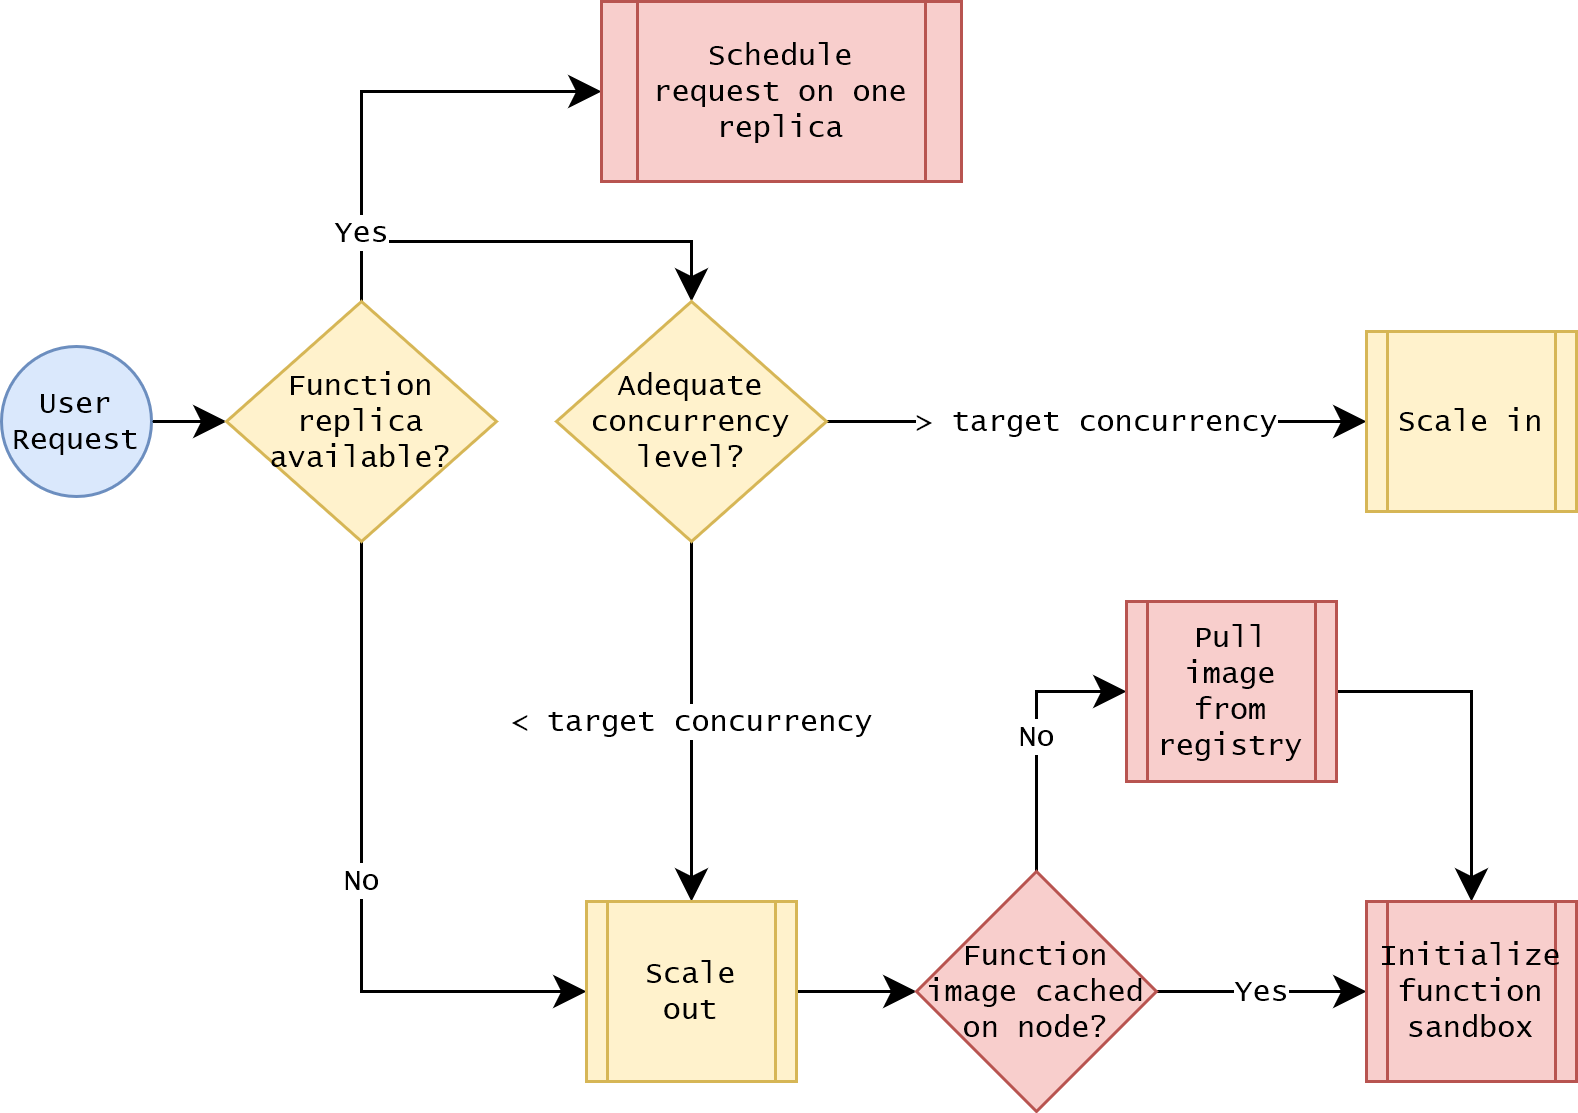
\includegraphics[width=0.8\columnwidth]{6_Chapitre4/figures/function-cache.png}
% \caption{Lifecycle of a user request in a serverless platform \jb{non référencée}}
% \label{figure:herocache-function-cache}
% \end{figure}

% \begin{figure}[t]
% \centering
% 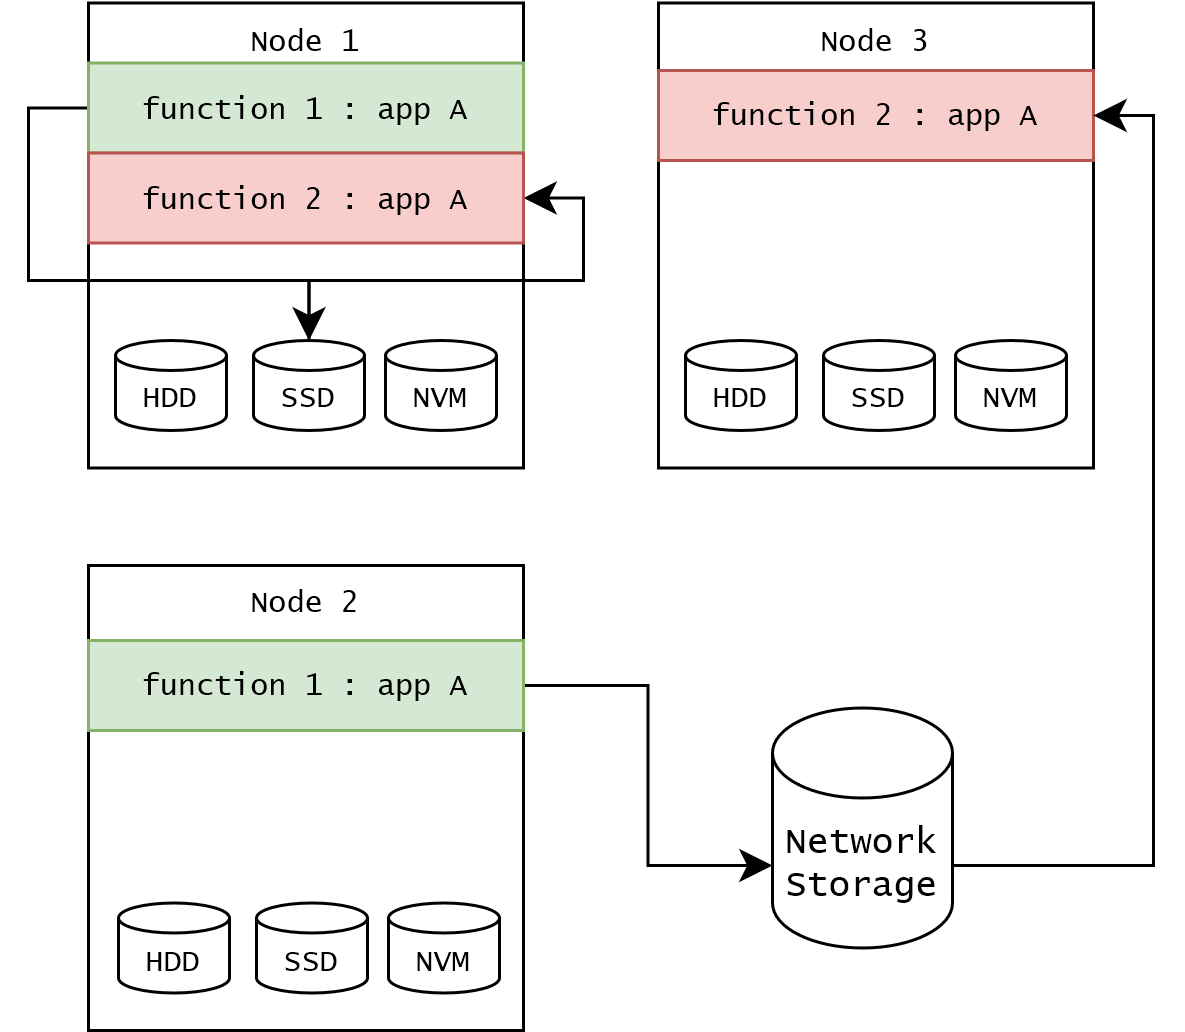
\includegraphics[width=0.8\columnwidth]{6_Chapitre4/figures/function-communications.png}
% \caption{Serverless functions communicate intermediate results through persistent storage that can be local to edge nodes or remotely accessible \jb{je ne vois pas l'interêt de cette figure non plus (le texte me semble suffire)}}
% \label{figure:herocache-function-communications}
% \end{figure}

\begin{figure*}[t]
\centering
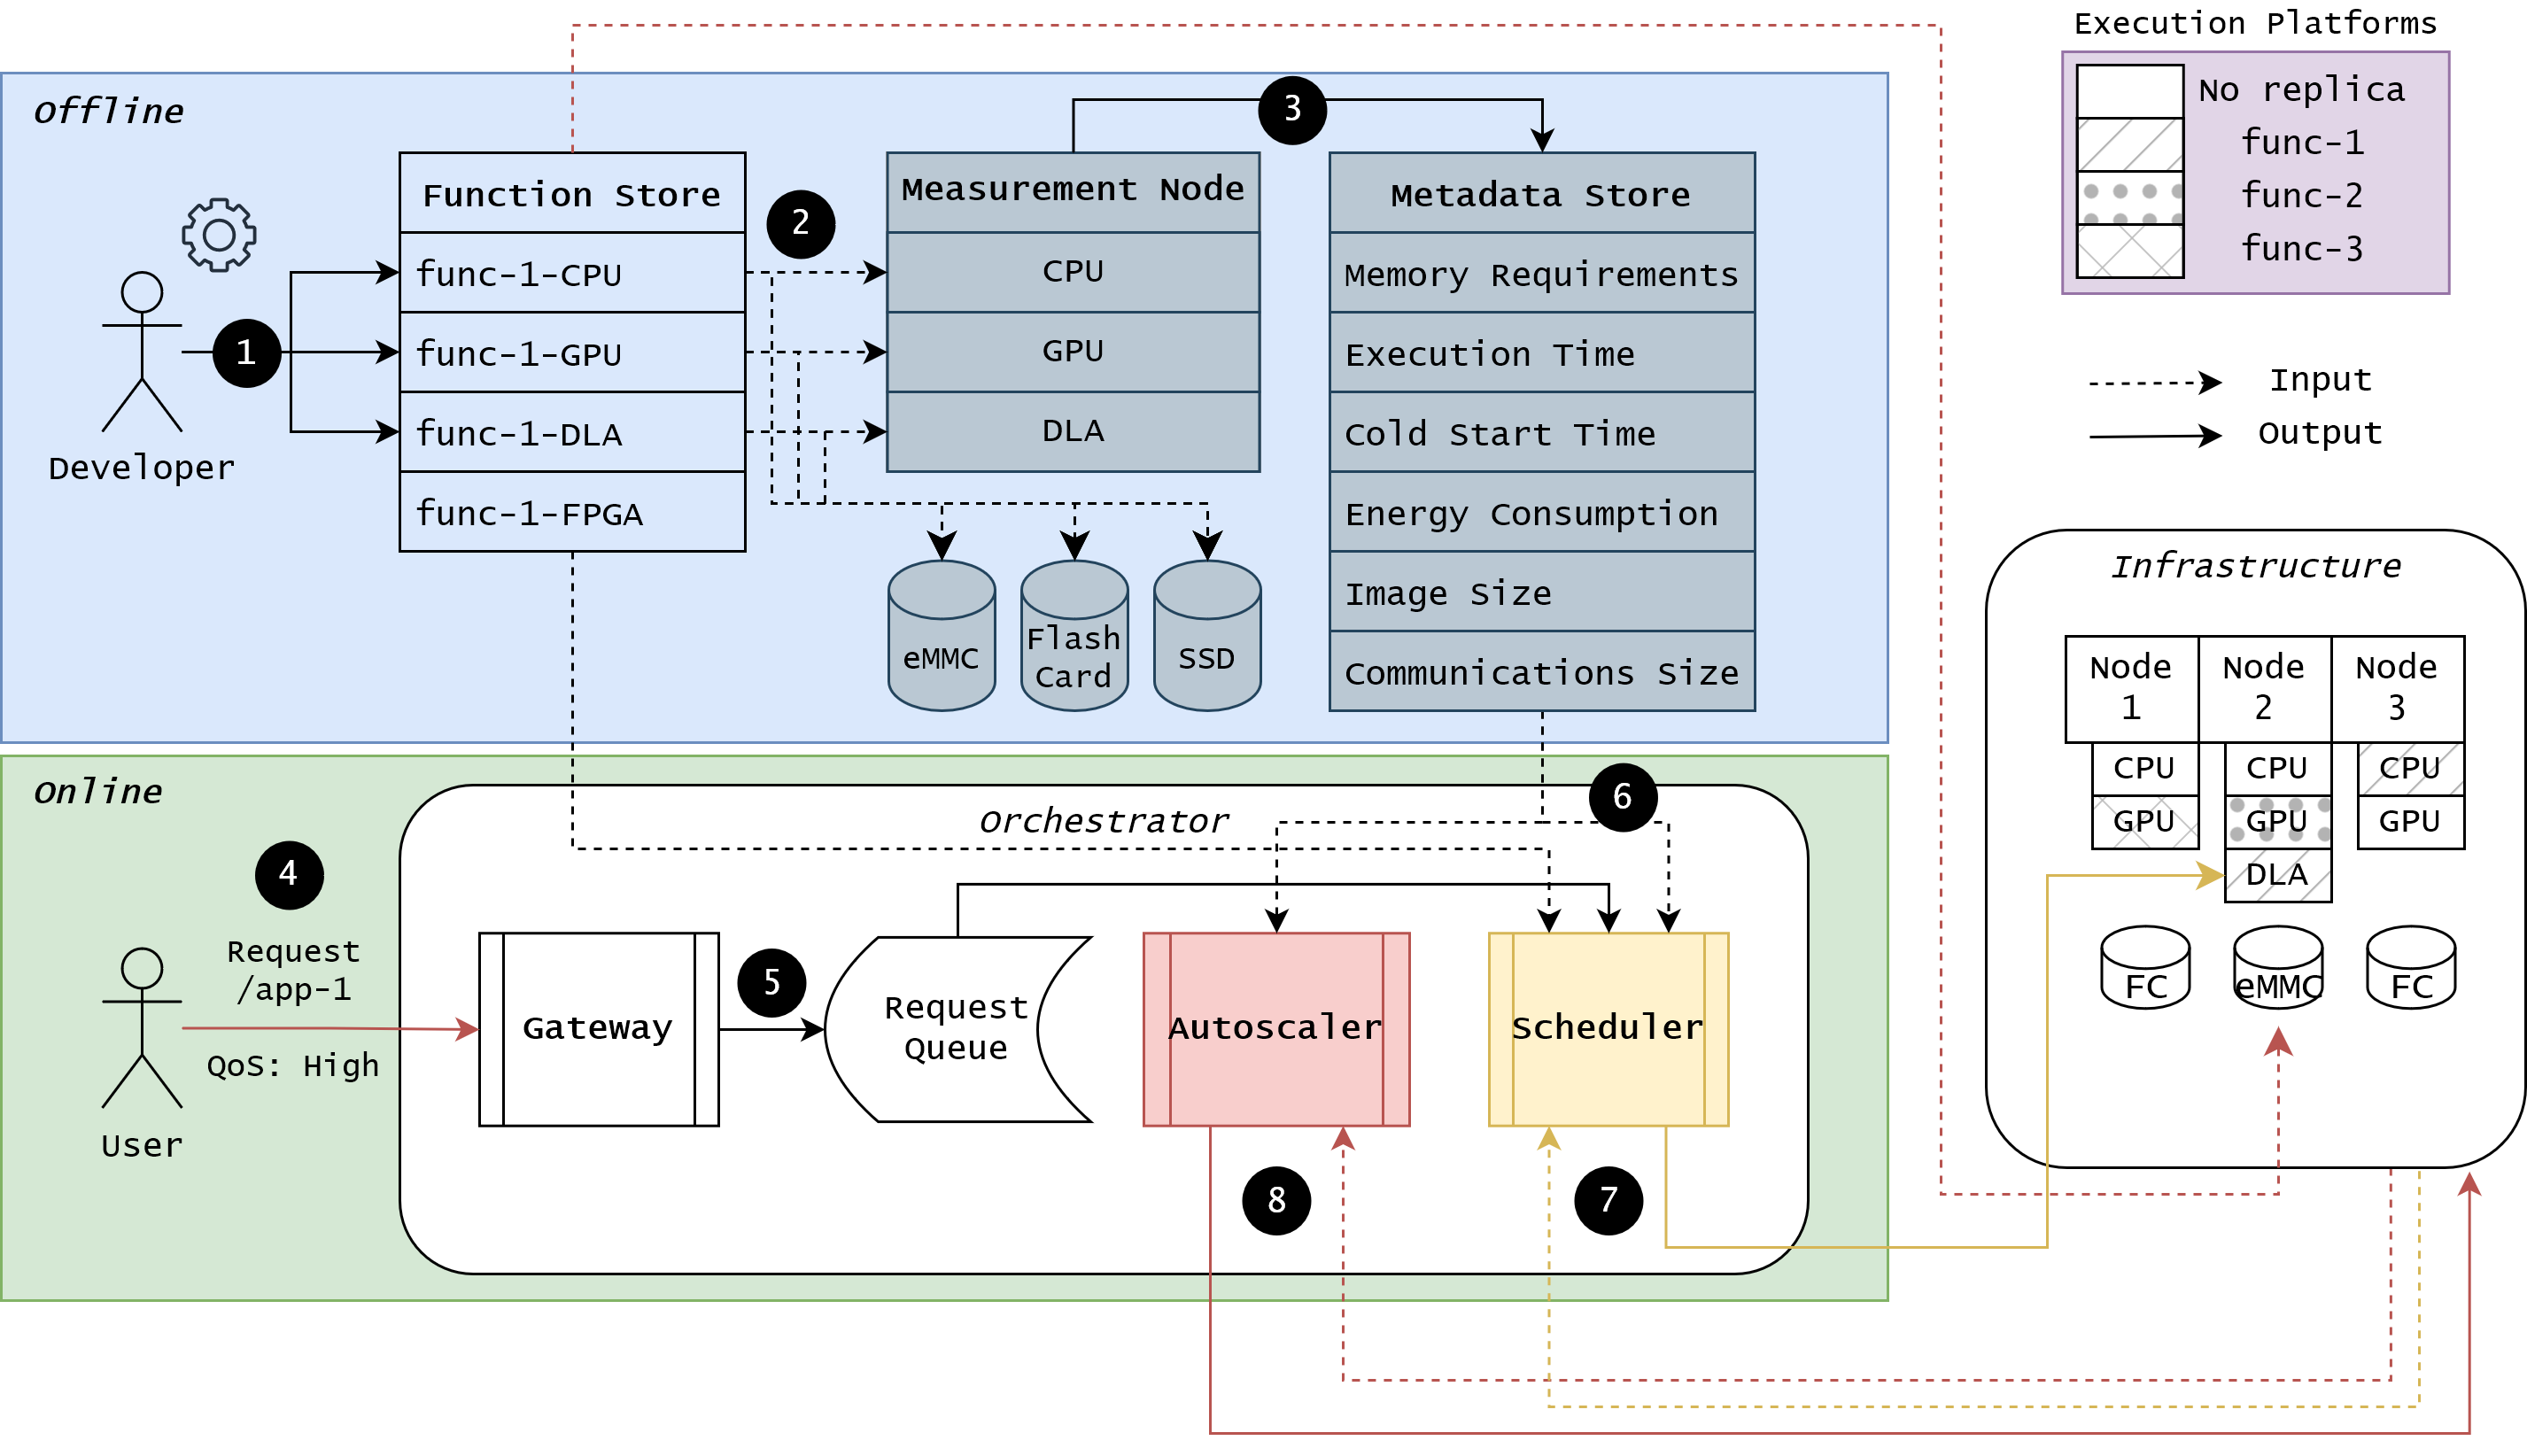
\includegraphics[width=0.65\textwidth]{6_Chapitre4/figures/serverless-platform-storage.png}
\caption{Serverless IDS platform, system overview}
\label{figure:herocache-serverless-platform}
\end{figure*}

%\subsection{Intrusion Detection Systems on the Edge}
%\label{section:herocache-background-ids}

%Because of the inherent criticality of the missions that can be performed by swarms of drones (industrial installation surveillance for example), 
% Being able to detect intrusion attempts early is a guarantee of a better responsiveness to threats and good progress of critical applications. Recent IDSs rely on resource-hungry ML models
%. Reaching satisfactory detection levels requires complex models with high memory and storage footprints, and significant calculation capabilities
% to perform traffic analysis within due time. In addition, the performance and energy consumption of the inference depends on 
%the complexity of the models and 
% the processing element on which they run. Yet, edge devices can be equipped with heterogeneous processing elements, making it possible to leverage these  resources and achieve a satisfying trade-off between security, performance and energy with respect to the conditions of the mission (criticality level, traffic load, battery level).

\subsection{Défis de l'orchestration dynamique}

Serverless is a trending service model for the cloud~\cite{Lannurien2023}: by shifting the resource allocation responsibility from customers to service providers, it alleviates an important part of the complexity from application developers and opens new opportunities of optimization and cost control for the infrastructure manager.
In a serverless architecture, developers design their applications as a composition of stateless functions. Stateless %(or "pure", side-effect free) 
means that the outcome of the computation depends exclusively on the inputs \cite{burckhardtNetheriteEfficientExecution}. These functions take a payload and an invocation context as input, and produce a result that is stored in a persistent network-accessible storage tier. %This means that data dependencies between functions in a chain have to be handled by the platform.

When an event triggers their execution, functions are deployed on nodes in the infrastructure, in execution environments called \textbf{replicas}. As functions are stateless, requests can be mapped to any available replica. Scaling a serverless application 
%\textit{i.e.} to maintain a consistent level of performance, 
consists in growing or shrinking the pool of replicas for the functions following the load peaks. Kubernetes-based serverless platforms such as Knative \cite{knative} or OpenWhisk \cite{openwhisk} proposed a threshold-based model for rightsizing the pool of replicas. For any function, an \textbf{autoscaler} can deploy multiple \textit{replicas} to absorb the load. Each replica is allocated on an execution platform (\textit{e.g.} one CPU core, one GPU, etc.) and has a request queue of fixed length for incoming requests. The number of replicas for a given function at any moment determines its concurrency level. A \textbf{scheduler} places user requests in queue on function replicas. When a replica has no more requests, it is deallocated. When a function is requested while no replica exists, it goes through a \textbf{cold start}.% that incurs an initialization delay to the function's response time.

%In serverless computing, the frequency of resource allocations dramatically increases compared to always-on, reserved resources environments such as IaaS offerings.
% The ability for serverless platforms to scale a function to zero replicas in order to avoid billing customers for idle resources is a key difference with regards to traditional cloud service models.
This cold start presents a risk of increased latency, as the provider has to allocate hardware resources and instantiate the application before responding to the request. The more complex the application, the higher the risk of large delays~\cite{mohanAgileColdStartsa}. Providers usually pre-allocate some resources to avoid cold starts, which comes with a cost in resources provisioning. Commercial actors such as AWS, Google and Microsoft all re-use function instances to some extent, keeping them running during a timeout period in order to circumvent latency costs incurred by cold starts~\cite{vahidiniaColdStartServerless2020}.

A recent study has shown that 50\% of serverless applications deployed at Microsoft Azure Durable Functions \footnote{\href{https://learn.microsoft.com/en-US/azure/azure-functions/durable/durable-functions-overview}{https://learn.microsoft.com/en-US/azure/azure-functions/durable/durable-functions-overview}} consist of 3 or fewer functions, with 65\% of the applications exhibiting a simple DAG of functions arranged as linear chains \cite{mahgoubORIONThreeRights}. Our IDS application consists of different chains that are two functions long, as described in Section~\ref{section:herocache-characterization-workloads}. Workload characterization work showed that 25\% of the functions deployed at Microsoft Azure Functions \footnote{\href{https://azure.microsoft.com/en-us/products/functions/}{https://azure.microsoft.com/en-us/products/functions/}} execute in 100 ms or less \cite{shahradServerlessWildCharacterizing}. The functions that make up our IDS application run for hundredths to tenths of a second, which makes them particularly prone to critical slowdowns in the context of dynamically allocated resources.

\subsection{Mise en cache des images de fonctions}
\label{section:herocache-background-cache}

% \vl{Cache} Online, dynamic resource allocation and task placement policies can help meet per-request Quality of Service (QoS) requirements by mapping the requests to appropriate replicas in the cluster. However, most papers on resources orchestration and task placement in serverless computing only consider best-case scenarios in which function images are already available on edge nodes. This does not reflect the reality, where function images are stored in repositories on dedicated nodes and pulled by worker nodes where and when functions are deployed. Depending on image size, this can have detrimental consequences on request latency with deployments where cold starts dominate a function's total response time \cite{yanHermesEfficientCache2020}. \jb{y a moyens de rendre le pb plus pertinent dans le cadre d'edge devices}

% In order to accommodate user requests without degrading performance, the autoscaler periodically adjusts the number of replicas for each deployed function: the replica pool grows and shrinks according to variations on the application's load. When load on a function increases beyond the platform's concurrency threshold, the autoscaler creates a new replica that will handle further user requests. When load decreases, idle replicas are removed. If there are no more requests for a given function, it can be \textit{scaled to zero}, effectively preventing resource waste.

Function replicas are initialized from \textbf{function images} (\textit{e.g.} a Docker image). These are stored in an image registry. Such registries can be remotely accessible through the Internet. %, but are mostly deployed in the provider's infrastructure in the context of a private cloud. 
However, numerous previous studies \cite{bhasiCypressInputSizesensitive2022, zijunFassflowEfficient2022, smithFaDOFaaSFunctions2022, zhangFIRSTExploitingMultiDimensional2023} only consider best-case scenarios in which function images are already available on edge nodes. This does not reflect the reality where function images are stored in registries on dedicated nodes and pulled by edge nodes where and when functions are deployed. %Depending on image size, this can have detrimental consequences on request latency in case where cold starts dominate a function's total response time.

In fact, pulling images on the edge nodes can account for more than 80\% of function response time \cite{yanHermesEfficientCache2020} since the cold start latency dominates the function's total response time. This is not acceptable when the platform has to meet stringent QoS requirements, as is the case for critical tasks such as IDS.

% To prevent this issue, %pulling these images over the network in further deployments, 
% function images can be cached on storage devices on the edge nodes, dramatically speeding up the process of deploying new instances of the function in the future. However, edge-node-local storage is limited in capacity and cannot be employed for caching purposes only. \jb{faire attention à ce que l'on dit ici, si le cache est une solution de l'état de l'art, il faudrait dire ce que l'on fait de mieux, sinon, si c'est une contrib, cela n'a rien à faire ici ...}

% Creating a replica thus implies pulling the image from the registry to the worker node. The image can then be cached on the worker node for use in further deployments, dramatically speeding up the process of spinning new instances of the function \cite{yanHermesEfficientCache2020}. However, node-local storage is limited in size and cannot be employed for caching purposes only.

\subsection{Communications entre les fonctions}
\label{section:herocache-background-communications}

% \vl{Communications} Furthermore, as these functions are sometimes scaled from zero, they are not network-addressable: inter-function communications are achieved through the use of slow, network-accessible storage (\textit{e.g.} S3 buckets). This induces delays that can snowball throughout the execution of the application and provoke Service Level Objective (SLO) violations by increasing request tail latencies \cite{wawrzoniakBoxerDataAnalytics2021a}. FaaS offerings are a typical example of data-shipping architecture: gigabytes of data are moved to megabytes of code, leading to inefficiencies that increase energy consumption and resource under-utilization. Ideally, functions that are part of a same application should be able to communicate intermediate results locally, using node-local storage rather than remote storage.

%Serverless functions are inherently \textit{stateless}, %which means that any request to a function can be handled by any replica in the infrastructure. This 
As it is necessary to support dynamic scaling of the functions, each invocation of a serverless function is self-contained and does not carry information or context from previous invocations. This allows replicas to queue user requests and handle them sequentially without the need to go through a cold start between requests. This introduces a constraint on the serverless platform: if an application is composed of several functions that form a processing pipeline, the output of each function must be stored in persistent storage to be fed as input to the next function in the chain~\cite{mullerLambadaInteractiveData2020}.

State-of-the-art work showed that serverless functions that communicate through remote storage can suffer up to 11x slowdown compared to functions using direct communications \cite{wawrzoniakBoxerDataAnalytics2021a}. The functions of our IDS application need to communicate intermediate results at each stage of the application's DAG. When functions are deployed on different edge nodes, inter-function communications will have to be achieved through the use of remote storage. This introduces slowdowns that can %snowball throughout the execution of the application and 
deteriorate QoS.

% Ideally, functions that are part of a same application should be able to communicate intermediate results locally, using node-local storage rather than remote storage. \vl{But storage is limited in performance and capacity on edge nodes, resulting in potential bottlenecks...}

% \subsection{Problem justification}

% \vl{Application characteristics:}

% \textbf{Function chains}. A recent study has shown that 50\% of serverless applications deployed at Microsoft Azure Durable Functions \footnote{\href{https://learn.microsoft.com/en-US/azure/azure-functions/durable/durable-functions-overview}{https://learn.microsoft.com/en-US/azure/azure-functions/durable/durable-functions-overview}} consist of 3 or less functions, with 65\% of the applications exhibiting a simple DAG of functions arranged as linear chains \cite{mahgoubORIONThreeRights}. Our IDS application consists in different chains that are two functions long, as shown in Figure~\ref{figure:herocache-ids-application}.

% \textbf{Short-running functions}. Workload characterization work showed that 25\% of the functions deployed at Microsoft Azure Functions \footnote{\href{https://azure.microsoft.com/en-us/products/functions/}{https://azure.microsoft.com/en-us/products/functions/}} execute in 100 ms or less \cite{shahradServerlessWildCharacterizing}. The functions that make up our IDS application run for hundredths to tenths of a second, which make them particularly prone to critical slowdowns in the context of dynamically allocated resources.

% \vl{Platform characteristics:}

% \textbf{Remote storage communications}. State of the Art work showed that serverless functions that communicate through remote storage can suffer up to almost 11x slowdown compared to functions using direct communications \cite{wawrzoniakBoxerDataAnalytics2021a}. The functions of our IDS application need to communicate intermediate results at each stage of the DAG.

% \textbf{Pulling function images}. Pulling the images on worker nodes can account for more than 80\% of function response time \cite{yanHermesEfficientCache2020}. This is not acceptable when the platform has to meet stringent QoS requirements, as is the case for mission critical tasks such as IDS. \vl{+ limited edge storage}

% Orchestrating serverless applications while achieving SLA thus requires carefully modeling application characteristics, and taking these into account when allocating resources and scheduling user requests on the serverless platform.

\section{Détection d'intrusion à l'edge dans le modèle serverless}
\label{section:herocache-before-contrib}

Orchestrating serverless applications while achieving SLA requires carefully modeling application characteristics and taking these into account when allocating resources and scheduling user requests on the serverless platform. Figure~\ref{figure:herocache-serverless-platform} gives an overview of the overall lifecycle of a request on our serverless platform. It is divided in two phases; an \textbf{offline phase} that consists in characterizing the applications deployed by the users on edge platforms, and an \textbf{online phase} where the requests to these applications are scheduled on the platform.

\textbf{Offline phase}. In our platform, the lifecycle of the application starts during an offline phase, where the developer provides the code for their functions for different hardware architectures (GPU, CPU, DLA, etc.)~\Circled{1}. This code is stored by the service provider in a function registry. The functions are then deployed on a measurement node~\Circled{2} where they are run to generate metadata relative to the execution of the functions on heterogeneous edge nodes. Memory requirements, execution time, cold start time, energy consumption, function size, and communication size for each function are written to a metadata store~\Circled{3}. Running the offline phase is required once for a given function on a given platform, as described in Section~\ref{section:herocache-workload}.

\textbf{Online phase}. Requests are sent to the IDS applications with a payload of TCP traffic (serialized packets) to analyze~\Circled{4}, and an associated desired QoS level for request response time. The request is appended to a request queue~\Circled{5} at the orchestrator level. When the scheduler pops the request from the queue, the metadata store is queried to retrieve the appropriate function metadata~\Circled{6}.

The scheduler will then try to find an available replica of the first function in the application to handle the request~\Circled{7}. If such a replica does not yet exist, the autoscaler will be asked to initialize a new instance of the function~\Circled{8}. During the lifecycle of the application, the autoscaler periodically checks the average load of each function to adjust the number of replicas deployed on the platform, depending on the concurrency threshold set by the service provider.

When the application completes, it returns a classification vector to the user that gives the probabilities that the traffic is malicious, exhibiting patterns of a potential attack.

\section{Phase hors-ligne : caractérisation} 
\label{section:herocache-workload}

% \begin{figure}[t]
% \centering
% 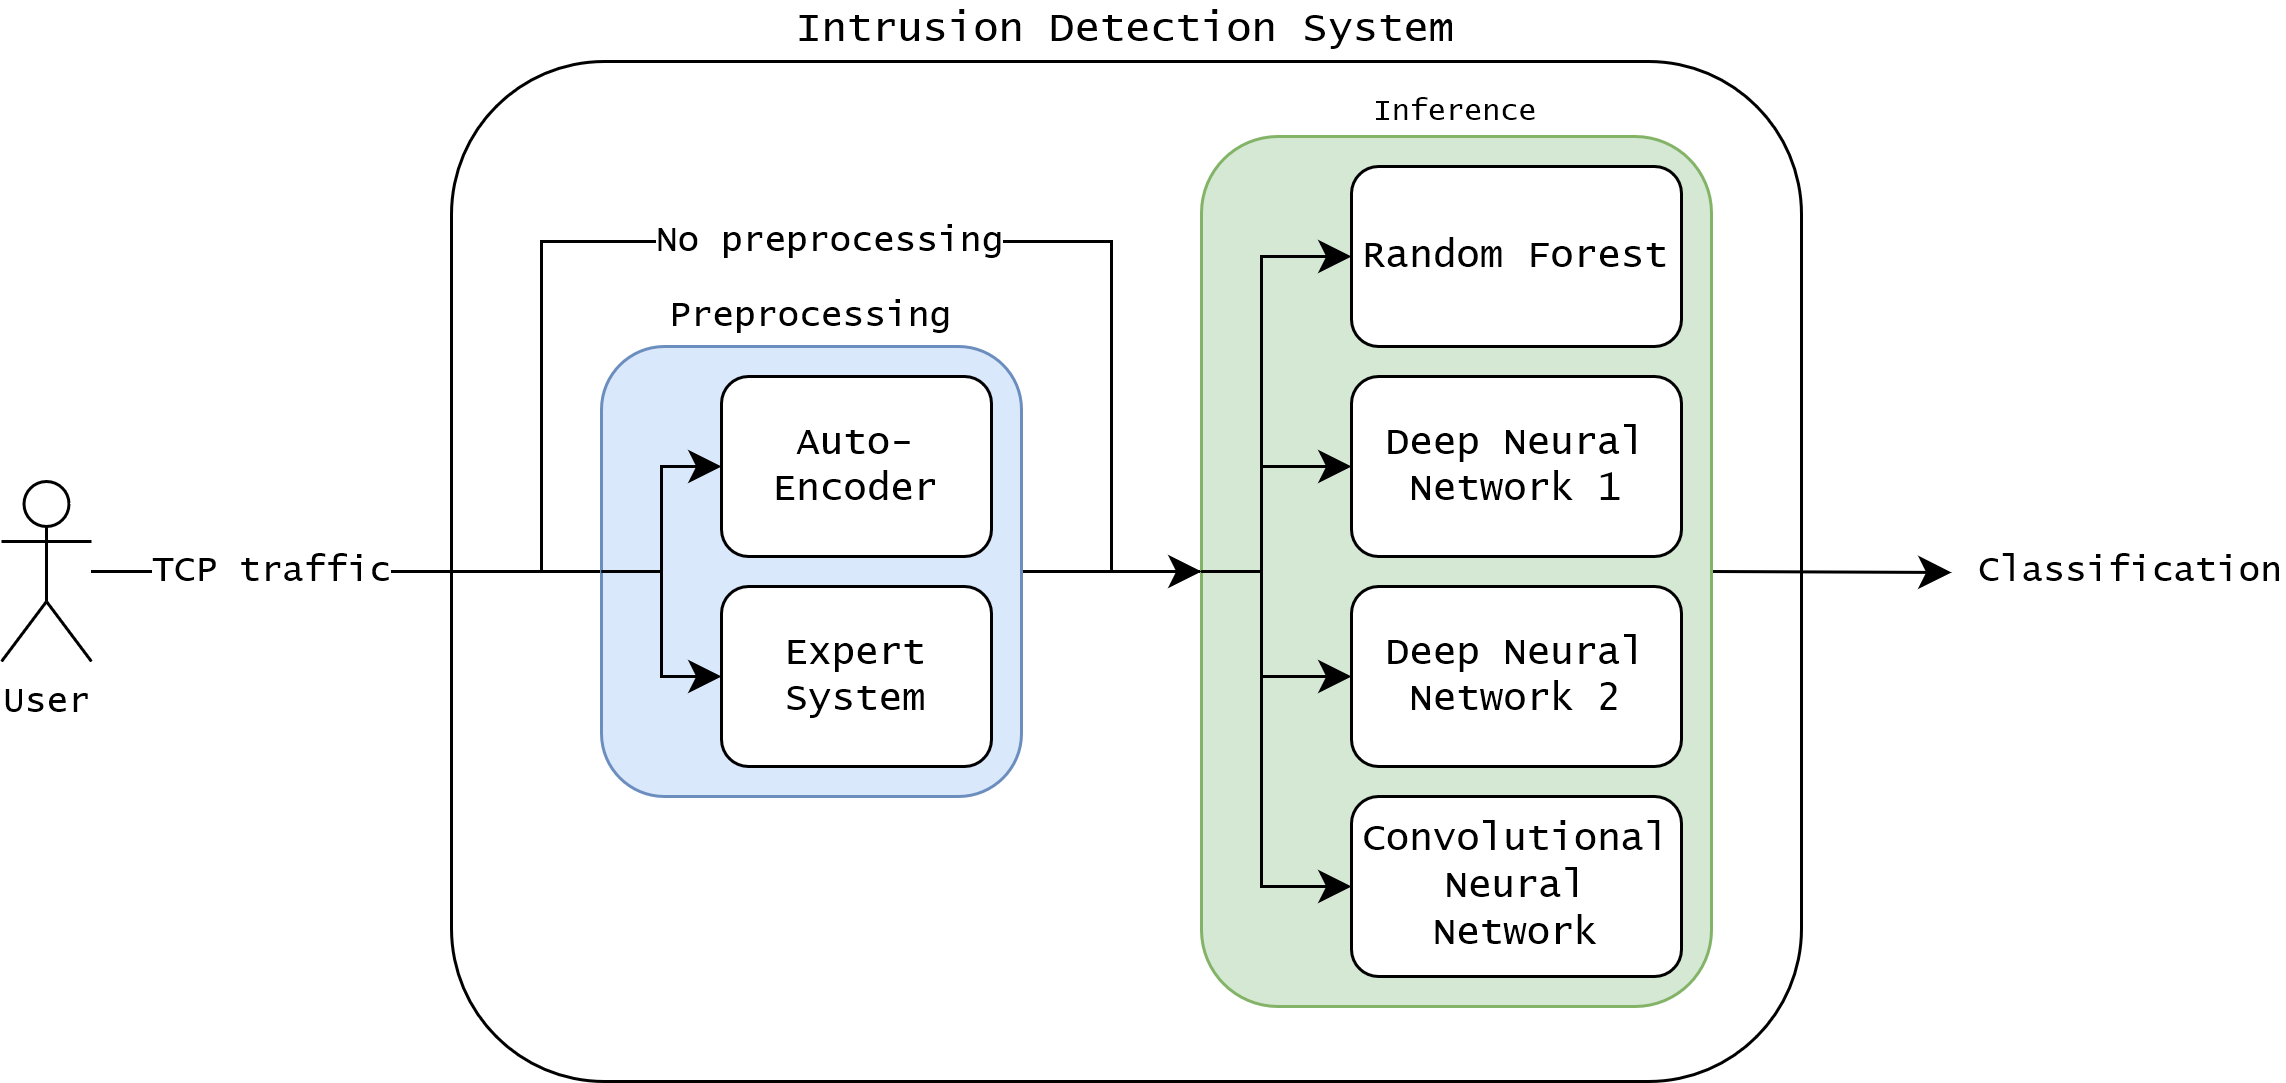
\includegraphics[width=0.8\columnwidth]{6_Chapitre4/figures/ids-application.png}
% \caption{Architecture of an IDS application that can make use of different preprocessing functions, and different inference functions to provide the user with a classification of TCP traffic \jb{cette figure n'apporte pas grand chose, en partie redondante avec la table 2}}
% \label{figure:herocache-ids-application}
% \end{figure}

%IDS are mandatory in critical and communication verbose systems, which is the case of swarms of drones. IDS rely on machine learning models that are energy hungry and time consuming. A conventional method of inference execution is to transfer observation data from collection devices into remote powerful servers. Nonetheless, this approach gives rise to privacy concerns and communication latency and energy overheads~\cite{ei-white-paper}. To address these issues, edge intelligence pushes machine learning models in proximity of collection devices, on low-performance and low-capacity devices. \jb{paragraphe précédent hors sol rien à voir avec le papier à sucrer}.

%A fine allocation of resources is necessary for IDS deployment on edge devices. 
A preliminary stage of platform and workload characterization is necessary to achieve adequate resource allocation and task placement for the execution of IDS models. To this end, we benchmarked several IDS models in terms of performance and energy on heterogeneous edge platforms that are representative of edge devices \cite{kljucaric2020}. %Such metrics are crucial for an efficient orchestration on top of heterogeneous edge platforms. 
This section describes our methodology and results.

%The authors characterized their models in terms of detection accuracy, latency, energy consumption and memory and storage footprints on different platforms and processing elements: Raspberry Pi 4 (CPU), Nvidia Jetson Xavier AGX (CPU, GPU and DLA) and a Pynq-Z2 FPGA.

\subsection{Caractérisation des plateformes d'exécution} \label{section:herocache-characterization-platforms}

We used platforms that are representative of what one can find in the edge~\cite{slimani:hal-04159551,kljucaric2020}: 
\textbf{(1) Raspberry Pi 4B} equipped with a quad core ARM Cortex-A72, 4 GB LPDDR4 main memory and a 16GB SD Card. It runs on Linux Raspbian 5.4.
\textbf{(2) Nvidia Jetson Xavier AGX} composed of three processing elements: an 8 core NVIDIA ARM Carmel CPU, an NVIDIA Volta GPU with 512 CUDA cores, and a Deep Learning Accelerator (DLA), which is a fixed-function hardware accelerator designed for Convolutional Neural Networks (CNN). It is assumed to be more energy efficient than the GPU. The NVIDIA Xavier AGX is equipped with 16 GB LPDDR4 and a 32 GB eMMC 5.1 Flash Storage. It runs on Linux Tegra 4.9.10. The 15 Watts Desktop power mode was used. 
\textbf{(3) PYNQ-Z2 Development Board}, a board based on the Xilinx Zynq XC7Z020 System on Chip. It is equipped with the Artix-7 FPGA and 512 MB DDR3 memory and a 16GB SD card.

\subsection{Caractérisation des applications}
\label{section:herocache-characterization-workloads}

Our application consists of different preprocessors and classifiers. The preprocessor selects a subset of relevant features of the TCP packets. 3 different preprocessing approaches were used: (1) using all the packet features without any selection (NoFS: No Feature Selection); (2) using a DNN auto-encoder to project features in a smaller latent space (AE: Auto-Encoder); and (3) expertly selecting a subset of the features (ES: Expert Selection). For the classifier part, we used Random Forest (RF), two different Dense Neural Network (DNN) architectures, and a CNN.

\begin{table}[t]
\caption{IDS models architectures and sizes}
\resizebox{\textwidth}{!}{
\begin{tabular}{|c|c|cc|}
\hline
Model     & Architecture                                                                                                                                         & \multicolumn{1}{c|}{Model Size on CPUs (MB)} & Model Size on GPU (MB) \\ \hline
NoFS-RF   & \begin{tabular}[c]{@{}c@{}}5 trees of 100\\ maximum depth\end{tabular}                                                                               & \multicolumn{1}{c|}{28}                      & 15.4                   \\ \hline
AE-RF     & \begin{tabular}[c]{@{}c@{}}5 trees of 50 \\ maximum depth\end{tabular}                                                                               & \multicolumn{1}{c|}{-}                       & 32.9                   \\ \hline
ES-RF     & \begin{tabular}[c]{@{}c@{}}10 trees of 10 \\ maximum depth\end{tabular}                                                                              & \multicolumn{1}{c|}{9.1}                     & 5.5                    \\ \hline
NoFS-DNN1 & \multirow{3}{*}{\begin{tabular}[c]{@{}c@{}}4 Dense Layers \\ (128x64x32x10)\end{tabular}}                                                            & \multicolumn{2}{c|}{0.144}                                            \\ \cline{1-1} \cline{3-4} 
AE-DNN1   &                                                                                                                                                      & \multicolumn{2}{c|}{0.321}                                            \\ \cline{1-1} \cline{3-4} 
ES-DNN1   &                                                                                                                                                      & \multicolumn{2}{c|}{0.053}                                            \\ \hline
NoFS-DNN2 & \multirow{3}{*}{\begin{tabular}[c]{@{}c@{}}5 Dense Layers \\ (7024x704x288x64x10)\end{tabular}}                                                      & \multicolumn{2}{c|}{3.33}                                             \\ \cline{1-1} \cline{3-4} 
AE-DNN2   &                                                                                                                                                      & \multicolumn{2}{c|}{2.96}                                             \\ \cline{1-1} \cline{3-4} 
ES-DNN2   &                                                                                                                                                      & \multicolumn{2}{c|}{2.61}                                             \\ \hline
NoFS-CNN  & \multirow{3}{*}{\begin{tabular}[c]{@{}c@{}}2 Conv1D (x64) - MaxPool \\ 3 Conv1D (x256) - MaxPool\\ 3 Dense Layers (100x20x10)\end{tabular}} & \multicolumn{2}{c|}{4.77}                                             \\ \cline{1-1} \cline{3-4} 
AE-CNN    &                                                                                                                                                      & \multicolumn{2}{c|}{2.9}                                              \\ \cline{1-1} \cline{3-4} 
ES-CNN    &                                                                                                                                                      & \multicolumn{2}{c|}{2.6}                                              \\ \hline
\end{tabular}
}
\label{table:herocache-workload}
\end{table}

Table~\ref{table:herocache-workload} shows the IDS models considered in this study and some of their characteristics. These models were trained and characterized on the reference network intrusion dataset UNSW-NB15\footnote{\href{https://research.unsw.edu.au/projects/unsw-nb15-dataset}{https://research.unsw.edu.au/projects/unsw-nb15-dataset}}
where each observation represents statistical, content and time features on data traffic during a time window, and tagged as "normal" or "attack". The dataset includes 9 attack categories. The neural network models were exported and optimized using TensorFlow Lite and TensorRT when intended for CPU and GPU/DLA platforms, respectively. Regarding Random Forest, the models were exported using the Emlearn and HummingBird.ml frameworks when targeting CPU and GPU platforms, respectively. hls4ml was used to export neural network models for the FPGA target.

\subsection{Mesures de performances}

Each of the IDS models was deployed on the target platforms and inferences were run with a set of 80,000 packets from the UNSW-NB15 dataset to characterize inference latency. The results are shown on Figure~\ref{figure:herocache-performance}. Only one model (ES-DNN1) has been characterized on the FPGA platform since the other HLS models could not be accommodated on the target. %the result has not been included in the figure \jb{pourquoi pas??}. Inferences on the FPGA processing element take 453 ms. 
The conclusion that was drawn from these results is that for neural networks, the Xavier CPU achieves the best performance in the majority of cases, except for NoFS-CNN which takes advantage of the GPU capabilities due to its high number of parameters and GPU efficiency for convolution operations. For Random Forest models, the fastest processing element is the GPU. In terms of cost and availability, the Xavier AGX is respectively around 20x and 10x more expensive than the RBPI4 and the Pynq-Z2 platforms, respectively. We size our infrastructure accordingly by providing more RBPI4 platforms than Xavier AGXs to be  representative of real deployments. % platforms than , even if its timing performances are better.

\begin{figure}
    \centering
    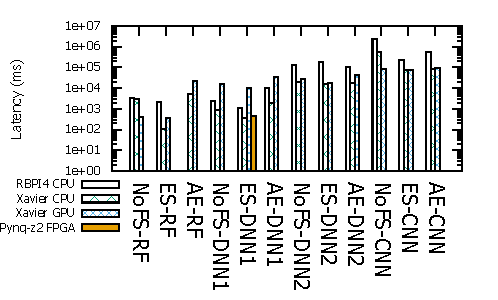
\includegraphics[width=0.9\columnwidth]{6_Chapitre4/figures/latency_bar.pdf}
    \caption{Latency characterization of IDS models}
    \label{figure:herocache-performance}
\end{figure}

\subsection{Mesures de consommation d'énergie}

%As with the latency \jb{energy ??}\vl{done} 
We run inferences on IDS models on each processing element and measured the energy consumption of the platform using the N6705A DC Power Analyzer. The results are shown in Figure~\ref{figure:herocache-energy}. For the same reasons mentioned above, only ES-DNN1 was characterized on FPGA. %, we did not include this result in the figure \jb{pourquoi pas??}. The energy consumption of the PYNQ-Z2 platform when running ES-DNN1 is 0.863J which is the lowest energy consumption compared to all other models and platforms.
We observe that the CPU processing elements show a lower energy consumption than the GPU in the majority of cases. The only case where the GPU shows better results is when the speedup it achieves as compared to CPUs is high. For instance, this occurs for NoFS-CNN where RBPI4 CPU is more than 30x slower than GPU.  
%In terms of cost, these results reinforce the choice to make RBPI4 more available than the Xavier platform. 
Even if Pynq-Z2 shows the best energy efficiency with the ES-DNN1 model, since it is more expensive and exhibits a limited design genericity, we assume it less available than RBPI4.

\begin{figure}
    \centering
    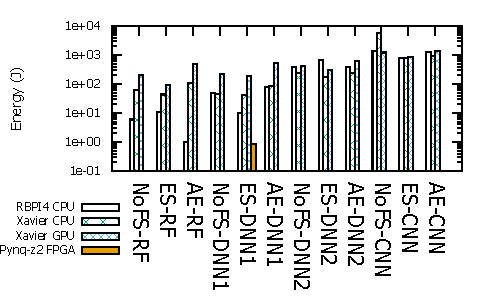
\includegraphics[width=0.9\columnwidth]{6_Chapitre4/figures/energy_bar.pdf}
    \caption{Energy characterization of IDS models}
    \label{figure:herocache-energy}
\end{figure}

\section{Phase en ligne : orchestration avec HeROcache} \label{section:herocache-contribution}

\subsection{Présentation générale}

The HeROcache orchestrator is mainly composed of two modules, the \textbf{autoscaler} and the \textbf{scheduler} (see Figure~\ref{figure:herocache-serverless-platform}). The autoscaler is in charge of dynamic resource allocation: it assigns execution platforms to function replicas. The scheduler handles the placement of user requests on the replicas.

HeROcache addresses the three above-mentioned challenges through the design of complementary greedy cost-minimization strategies at the autoscaler and scheduler levels. HeROcache minimizes \textbf{initialization delays} by considering the latencies of image extraction at the autoscaler level. Prefetching strategies are also implemented for function image caching. \textbf{Inter-function communication} costs are considered mainly in the scheduler part, which naturally tends to consolidate functions from the same application. The autoscaler participates indirectly in this consolidation by prefetching the next functions of the DAG of the application on the same edge node. Finally, \textbf{heterogeneous platforms} are taken into account as the different execution costs extracted during the offline phase (see Section~\ref{section:herocache-workload}) are considered throughout the entire autoscaling and scheduling process. %Indeed, the various levels of performance delivered by the heterogeneous hardware can result in different makespans for a given scenario. The energy consumption can vary depending on the hardware allocated to a replica. Furthermore, user requests do not require the same response time depending on the applications. %We argue that the serverless orchestrator has to be \textbf{cost-aware} to perform optimal decisions.
The next sections describe both the autoscaling and scheduling strategies. %present a formal description of our strategy for the autoscaling of resources and scheduling of applications.
\begin{table}[t]
    \caption{Notation dictionary}
    \begin{center}
    \scalebox{0.85}{\begin{tabularx}{\linewidth}{|c|Y|}
    \hline
    \textbf{Notation} & \textbf{Description} \\ \hline
    $x_a$ & Allocation of resource for application $a$ \\ \hline
    $y_a$ & Invocation of application $a$ \\ \hline
    $z_i$ & Placement of task for function $i$ \\ \hline
    $f_{N, P}$ & A function $f$ scheduled to run on a platform $P$ available on node $N$ \\ \hline
    $f_{a}$ & A function $f$ that belongs to application $a$ \\ \hline
    $A$ & Total number of applications to be scheduled on the platform \\ \hline
    $F_{a}$ & Total number of functions that belong to an application $a$ \\ \hline
    $RT_{{f}_{N, P}}$ & Time to retrieve function image for $f$ to run on a platform $P$ available on node $N$ \\ \hline
    $NB_{N}$ & Network bandwidth between node $N$ and the infrastructure \\ \hline
    $SMT_{N}$ & Storage medium throughput on node $N$ \\ \hline
    $SML_{N}$ & Storage medium latency on node $N$ \\ \hline
    $QP$ & QoS penalty \\ \hline
    $QD$ & QoS deviation \\ \hline
    $WET$ & Worst execution time \\ \hline
    $TT$ & Task total time \\ \hline
    $CST$ & Cold start time \\ \hline
    $ST$ & Storage time \\ \hline
    $ET$ & Execution time \\ \hline
    $EC$ & Energy consumption \\ \hline
    $IS$ & Image size \\ \hline
    $HP$ & Hardware price \\ \hline
    $TC$ & Task consolidation \\ \hline
    $Q$ & Task queue on a replica \\ \hline
    $CP$ & Cache proportion \\ \hline
    $SIS^{f}_{a}$, $SOS^{f}_{a}$ & Size of resp. input, output state of function $f$ that belongs to application $a$ \\ \hline
    % $replicaCount_{f, h}$ & Size of the replica pool for a function $f$ on hardware type $h$ \\ \hline
    % $concurrency_{f, h}$ & Average number of in-flight requests for a function $f$ on replicas of hardware type $h$ \\ \hline
    $threshold_{f, h}$ & Concurrency threshold for a function $f$ on a replica of hardware type $h$ \\ \hline
    $scaleCost^{{f}_{{i}_{N, P}}}_a$ & Cost of creating a new replica for function $f_i$ from application $a$ on a platform $P$ available on node $N$ \\ \hline
    $schedCost^{{f}_{{i}_{N, P}}}_a$ & Cost of scheduling an execution of function $f$ from application $a$ on a platform $P$ available on node $N$ \\ \hline
    \end{tabularx}}
    \label{table:herocache-notation}
    \end{center}
\end{table}

% \subsubsection{IDS Applications}

% We consider applications as the composition of tasks (function executions): an application is represented as a directed acyclic graph (DAG). Vertices are functions of the applications. Each edge carries data from one function to the next in the flow.

% % \begin{figure}[t]
% % \centering
% % 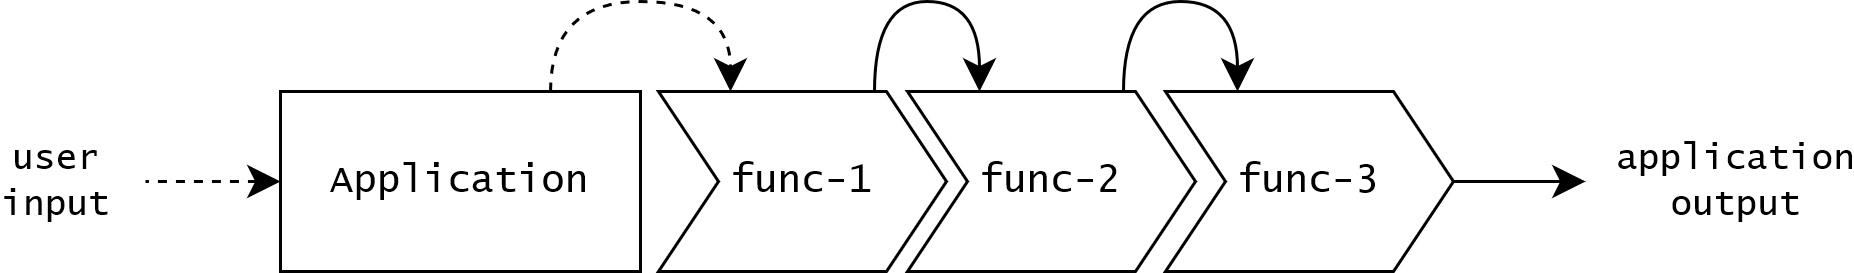
\includegraphics[width=0.8\columnwidth]{6_Chapitre4/figures/serverless-application.png}
% % \caption{A serverless application modeled as a function chain \jb{pas sur que c'est utile + pb sémantique on a une appli qui envoie les données à une fonction... des formes diff et des fleches diff sans expliciter ... ce qui prendra encore plus de place, donc à mon avis, supprimer ... ou sinon à mettre à l'interrieur de la figure 3 celle du schéma global}}
% % \label{figure:herocache-serverless-application}
% % \end{figure}

% To schedule such an application on a serverless platform, its function chain must be scheduled by traversing the DAG. \jb{tu donnes un bout de contrib de manière isolé. IL serait peut être plus judicieux de dire ce à quoi on doit faire attention.}\vl{done} The platform must verify at each function invocation that their dependencies are met (\textit{i.e.} that all their predecessors have been successfully ran to completion). It must then retrieve their input data and finally schedule the request on an available replica.

% Functions are scheduled onto execution platforms (CPU, GPU, DLA) that belong to nodes (servers) in the infrastructure. Each function takes input data and produces a result as output data. Data are stored in storage devices (eMMC, Flash Card, SSD) that can either be local to the node or remotely available through the network.

% Serverless functions are basic building blocks that are re-used across applications. Applications are composed of a minimum of one function.

% \begin{figure}[t]
% \centering
% 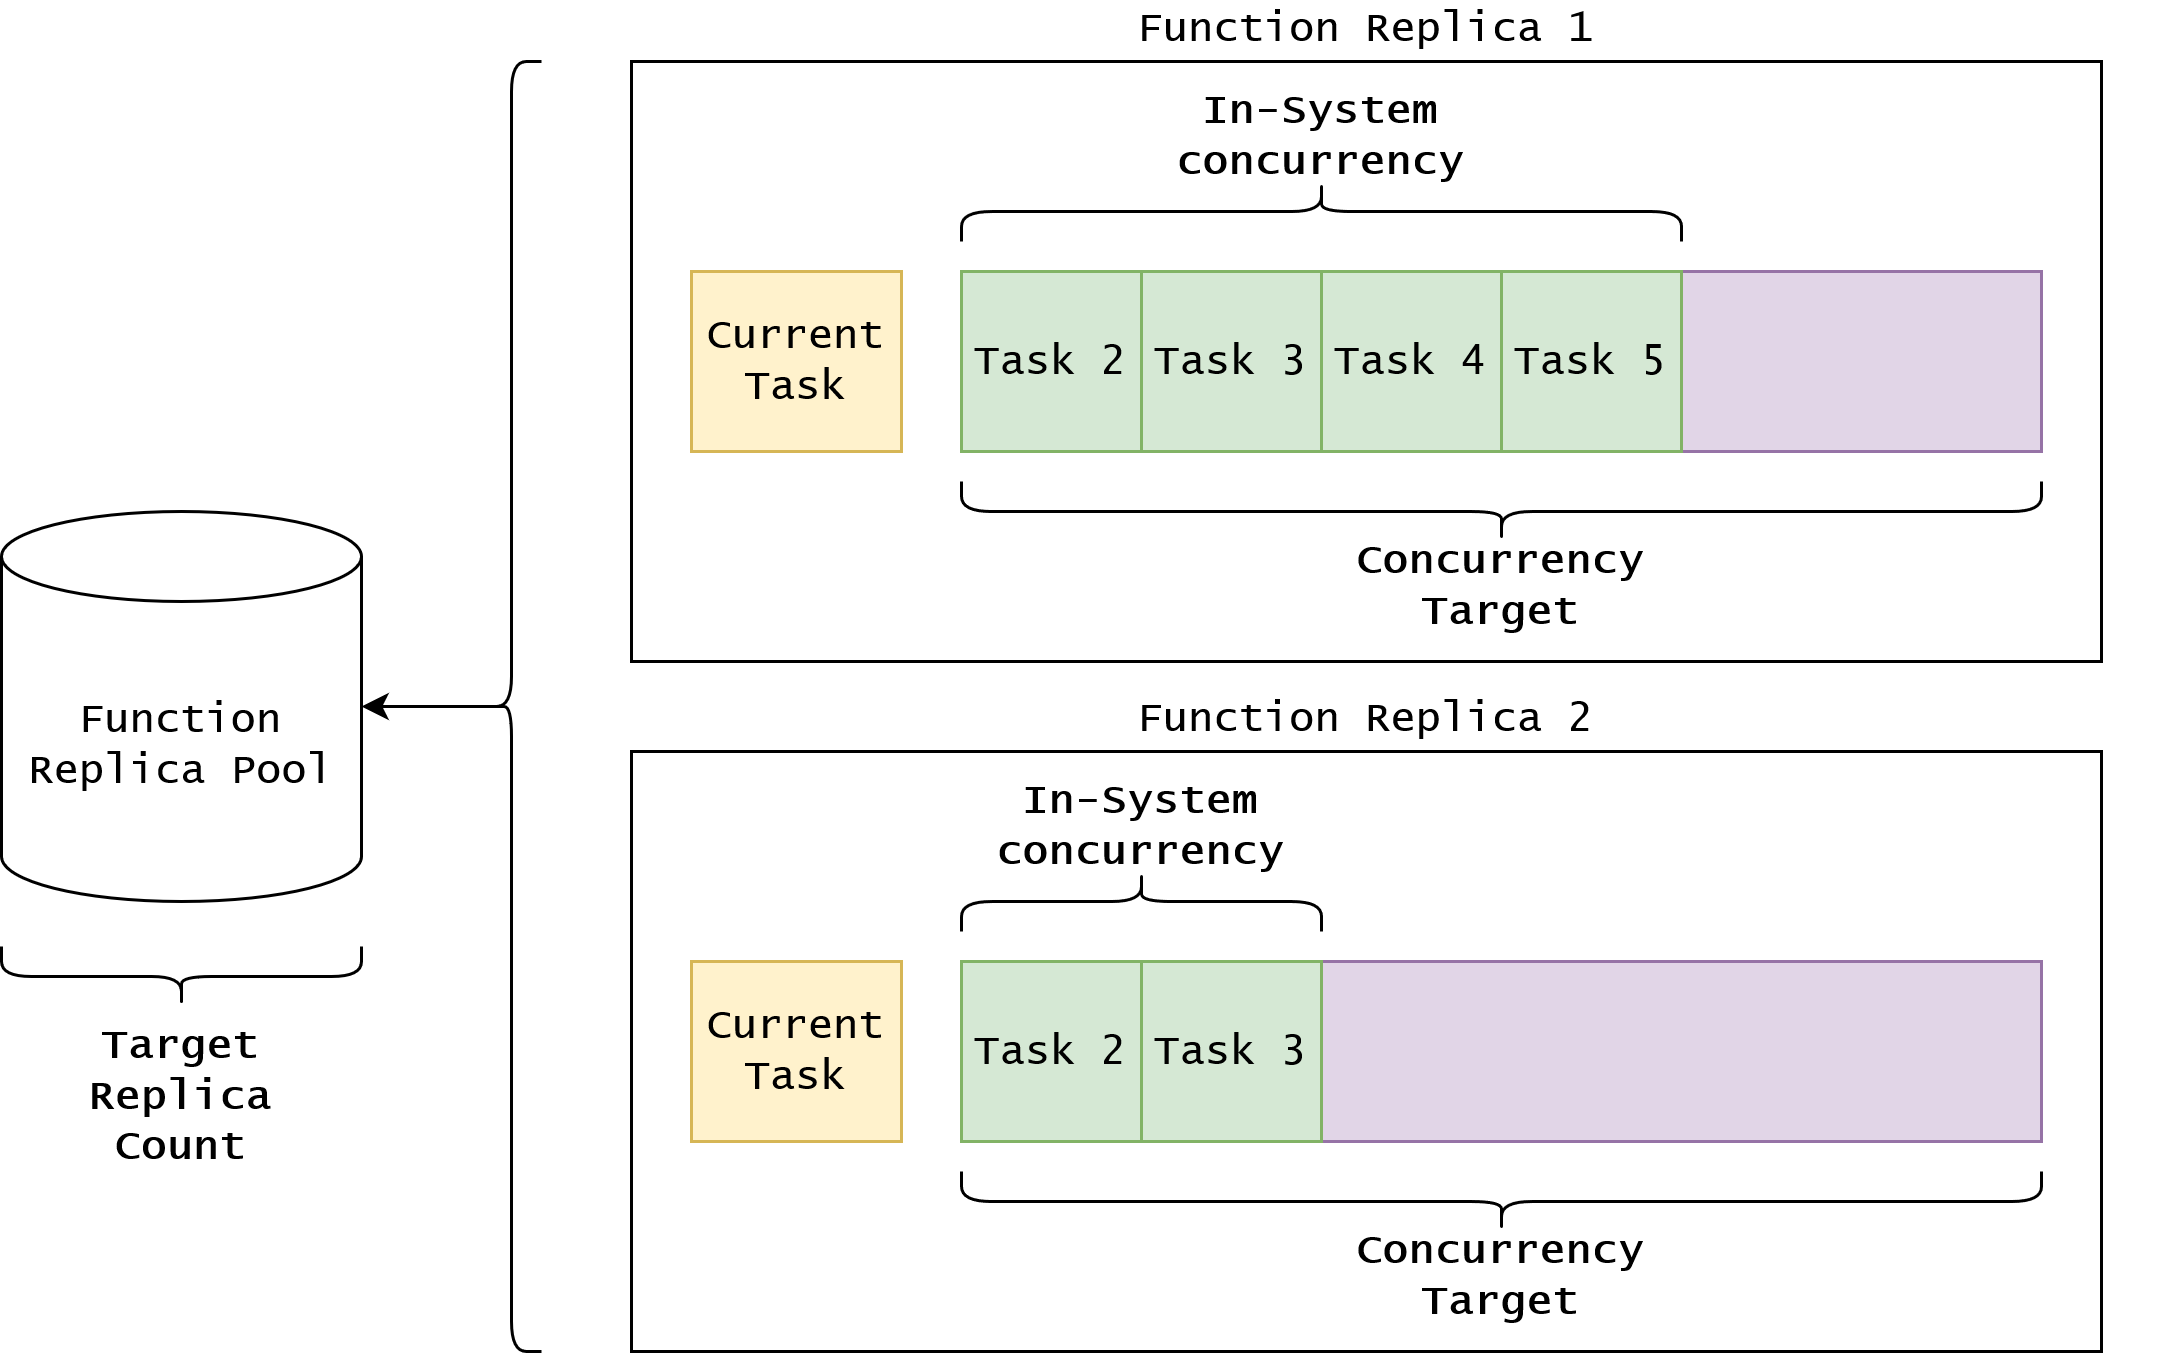
\includegraphics[width=0.8\columnwidth]{6_Chapitre4/figures/replica-count.png}
% \caption{Rightsizing dynamic allocations in a serverless platform requires defining an adequate number of function replicas, and the number of user requests that can be queued on each of these \jb{à discuter car pas explicite pour moi (il n'y a pas de plateforme !! et pas de "function" ... toujours les pb de terminologie} \vl{montrer des concurrency targets différentes en illustrant par le choix du matériel alloué à la réplique ?}}
% \label{figure:herocache-replica-count}
% \end{figure}

% \vl{à résumer et déplacer en background (idée importante : dimensionnement des répliques)}

% Our platform follows the threshold-based horizontal scaling model found in open-source, Kubernetes-based serverless platforms such as Knative \cite{knative} or OpenWhisk \cite{openwhisk}. For any function, an autoscaler can deploy $n$ \textit{replicas}. Each replica is allocated an execution platform (\textit{e.g.} one CPU core, one GPU, etc.) and has a request queue $Q$ of fixed length for incoming user requests. The number of replicas for a given function at any moment determines its concurrency level (Figure~\ref{figure:herocache-replica-count}).

% In Knative, the number of replicas for a given function (Equation~\ref{eq:herocache-replica-count}) depends on the moving average load for a function, \textit{i.e.} the average number of queued \jb{un mot plus simple ... queued? } requests for the function over a 60-second window. It is bounded by a concurrency threshold per replica, \textit{i.e.} the maximum number of requests queued in a function's replica at any moment. The default value in Knative is 100 in-flight requests in each replica~\cite{knative-autoscaling} \jb{pour moi le paragraphe précédent est incompréhensible on ne comprend ni l'intuition ni le comment}. In~\cite{herofake}, the authors proposed to allow better handling of hardware heterogeneity by the platform by setting a per-function type, per-hardware type scaling policy. The authors established a performance ratio between the CPU and the various hardware accelerators. In the present contribution, where we have multiple CPU types at hand, we build upon this mechanism and generalize it to any baseline platform by establishing the ratio with regard to the slowest platform $x$ (Equation~\ref{eq:herocache-performance-ratio}). The baseline concurrency threshold is to be fixed by the service provider; we discuss this value in our evaluation (Section~\ref{section:herocache-evaluation}).\jb{pas self contained car référence nécessaire au précédent papier ... pas bon ça}

% \begin{equation}
%     replicaCount_{f, h} = \, \frac{concurrency_{f, h}}{threshold_{f, h}}
% \label{eq:herocache-replica-count}
% \end{equation}

% \begin{equation}
%     threshold_{f, h} = \, threshold_{f, x} \cdot ratio
% \label{eq:herocache-threshold-baseline}
% \end{equation}

% \begin{equation}
% \resizebox{0.9\columnwidth}{!}{
%     $ratio = \, k_{CST} \cdot \frac{CST_{{f}_{x}}}{CST_{{f}_{h}}} + k_{ET} \cdot \frac{ET_{{f}_{x}}}{ET_{{f}_{h}}} + k_{EC} \cdot \frac{EC_{{f}_{x}}}{EC_{{f}_{h}}} + k_{HP} \cdot \frac{HP_{{f}_{x}}}{HP_{{f}_{h}}}$
% }
% \label{eq:herocache-performance-ratio}
% \end{equation}

\subsection{Stratégie de minimisation des coûts d'allocation des ressources}

%\vl{Il faudrait presque déplacer le paragraphe suivant, qui introduit la raison de formuler un problème d'optimisation, avant les 2 sections autoscaling cost / scheduling cost. Sinon, on dirait qu'il manque une introduction à la sous-section scheduling cost. Qu'en penses-tu ?}

%With a heterogeneous infrastructure, the orchestrator's allocation and placement decisions can produce very different results in terms of QoS. The various levels of performance delivered by the hardware can result in different makespans for a given scenario. The energy consumption can vary depending on the hardware allocated for a replica. Furthermore, user requests do not require the same response time, and are related to various applications. We argue that the serverless orchestrator has to be \textbf{cost-aware} to perform optimal decisions.

We formulate resource allocation as an optimization problem and solve it with a simple greedy algorithm. The objective of the autoscaler is to minimize the cost of the sum of allocations $scaleCost_{a}$ for $y_a$ invocations of application $a$ (Equation~\ref{eq:herocache-objective-allocation}) for all applications in $A$, under the constraint of a finite infrastructure with $x_a$ being the allocation of resources for application $a$ (Equation~\ref{eq:herocache-constraint-allocation}). 

\begin{equation}
    \forall A, \, \min \sum_{a = 0}^{A} y_a \cdot scaleCost_{a}
\label{eq:herocache-objective-allocation}
\end{equation}

\begin{equation}
    \text{s. t.} \, \sum_{a = 0}^{A} x_a \leq Total Resources
\label{eq:herocache-constraint-allocation}
\end{equation}

The cost of resource allocation for an application $a$ is the sum of the allocation costs for its functions (Equation~\ref{eq:herocache-scale-cost-app}). One replica is allocated to one execution platform.

\begin{equation}
    scaleCost_{a} = \, \sum_{i = 0}^{F_{a}} scaleCost^{{f}_{{i}_{N, P}}}_a
\label{eq:herocache-scale-cost-app}
\end{equation}

Each function replica has an associated allocation cost. %, as dynamically allocating hardware resources introduces latency while handling user requests. 

We designed a cost model (Equation~\ref{eq:herocache-scale-cost-function}) for the resource allocation needed to deploy one function of a given application. It is composed of four components, the sum of which we need to minimize:
%\jb{ici il faut dire ce que modélise chaque cout avant de parler d'objectif}
\begin{itemize}
    \item the \textit{cache proportion} $CP$ translates the scattering of the functions on the different edge nodes. The higher the score, the more scattered the functions on the nodes. Minimizing this term helps in consolidating the functions;
    \item the \textit{total time} $TT$ represents the total execution time of the function. It consider the QoS of the application, the heterogeneity of the platform and the deployment cost (whether the image is cached or distant). The higher this cost, the lower the QoS;
    \item the \textit{energy consumption} $EC$ translates the energy consumption of the function deployment. The higher $EC$, the higher the cost;
    \item the \textit{hardware price} $HP$ describes the Total Cost of Ownership (TCO) supported by service providers related to the execution time. This translates the cost of deployment on a given hardware platform. The higher $HP$ the higher the cost of the solution.
\end{itemize}

The overall objective of the cost model is to deploy a function with the lowest cost possible, that is an increased consolidation, a reduced makespan, a reduced energy consumption, and a reduced cost of ownership. We will detail each part of Equation~\ref{eq:herocache-scale-cost-function} in the next paragraphs. Each component of the equation is weighted to allow flexible tuning; the values we chose for the deployment of the IDS application are specified in the evaluation part (Section~\ref{section:herocache-evaluation}).

\begin{equation}
\begin{split}
 \forall N, \forall P \in N, scaleCost^{{f}_{{i}_{N, P}}}_{a} = \,   &k_{CP} \cdot {CP}_{{a}_{N}}    \\
    + &k_{TT} \cdot {TT}_{{f}_{N, P}} \\
    + &k_{EC} \cdot {EC}_{{f}_{N, P}} \\
    + &k_{HP} \cdot {HP}_{{f}_{N, P}}
\end{split}
\label{eq:herocache-scale-cost-function}
\end{equation}

% When the autoscaler considers scaling a function, it computes the proportion of function images from its application(s) cached on each available node. Note that at the autoscaler level, decisions are made at the granularity of a function -- not of an application. Thus, we compute the cache proportion for each application a function can belong to. The score is then averaged considering the number of applications that include the function. \jb{toujours pas bon car équation pas expliquée encore!!}

\textbf{Cache Proportion}. 
%The first delay introduced by dynamic allocation of resources occurs before replica initialization. The function image must be pulled on the node from a remote registry, which adds latency to the handling of the first request in replica queue. 
As seen earlier, enforcing task (a function execution) consolidation among applications should help minimize communication and delays in the function chains. HeROcache pushes toward deploying replicas of a function on nodes where other functions belonging to the same application are already deployed.

To do so, HeROcache keeps track of $CF_{a}^{{f}_{i_{N, P}}}$ the number of function images ${f}_{i}$ of application $a$ deployed on node $N$ on a given execution platform $P$ (e.g. GPU) available in cache on node-local storage. The proportion of cached functions is computed for each application (Equation~\ref{eq:herocache-cached-functions}) and then averaged over all applications running on a given node and inverted to give a high value for non-consolidated functions (as the objective is to minimize this proportion), see Equation~\ref{eq:herocache-cache-proportion-app}.

% \begin{equation}
%     \forall a \in A, \forall f \in a, \, Cached Functions{a}^{{f}_{i_{N, P}}} = \, 
% \label{eq:herocache-local-proportions}
% \end{equation}

%When the autoscaler considers scaling a function, it computes these $Cached Functions$ on each available node. Note that at the autoscaler level, decisions are made at the granularity of a function -- not of an application. Thus, we compute the cached proportion of functions for each application a function can belong to. The score is then averaged in the \textit{cache proportion} $CP$ considering the number of applications that include the function.
% We call this first component of scaling cost the \textit{cache proportion} (Equation~\ref{eq:herocache-cache-proportion-app}). % By considering this cache proportion in the allocation cost, we seek to consolidate functions of the same application on a limited number of nodes.

\begin{equation}
    \forall a \in A, \, \forall f \in a, \, CF_{a}^{{f}_{i_{N, P}}} = \frac{\sum_{i = 0}^{Fa} isCached(f_{i}, N, P)}{F_{a}}
\label{eq:herocache-cached-functions}
\end{equation}

\begin{equation}
    \forall N, \forall P \in N, \, {CP}_{{a}_{N}} = \, \frac{A}{\sum_{i = 0}^{F_{a}} CF_{a}^{{f}_{i_{N, P}}}}
\label{eq:herocache-cache-proportion-app}
\end{equation}

% \textbf{Image cache prefetching}.
In addition to the cost minimization, in order to reduce deployment delays, the autoscaler prefetches images for function chains when deploying a new replica on a node. It inspects function chains and sequentially pulls missing function images from the remote registry to node-local storage asynchronously. %When the pulling of the images on the node is over and new replicas of these functions are created, the autoscaler will benefit from an initialization delay reduction on that node. 
% \textbf{Cache eviction}.
%When node-local cache is filled, we enforce a simple FIFO replacement policy.

\textbf{Total Time}. The second component of scaling cost is the \textit{total time}. Minimizing total time should prevent initialization delays snowballing throughout function chains, thus preventing SLA violations.

Thanks to the metadata collected about each function during the offline phase, the autoscaler is able to predict the time to completion $ {TT}_{{f}_{N, P}}$ of the first request that will be scheduled onto a new function replica (Equation~\ref{eq:herocache-total-time-function}).

\begin{equation}
    {TT}_{{f}_{N, P}} = \, {RT}_{{f}_{N, P}} + {WT}_{{f}_{N, P}} + {CST}_{{f}_{N, P}} + {ET}_{{f}_{N, P}}
\label{eq:herocache-total-time-function}
\end{equation}

\begin{itemize}
    \item ${RT}_{{f}_{N, P}}$ is the duration of the image retrieval time of the function. If the function's image is already cached on the compute node, this duration is zero; otherwise, it depends on the image size $IS$ and is influenced by the network link bandwidth $NB$, as the image will be read from a remote image registry, and by the node storage medium throughput $SMT$ and latency $SML$, as the image will be written and stored locally for further use (Equation~\ref{eq:herocache-retrieval-time});

    \begin{equation}
        {RT}_{{f}_{N, P}} = \, \frac{IS_{{f}_{N, P}}}{\min (NB_{N}, SMT_{N})} + SML_{N}
        \label{eq:herocache-retrieval-time}
    \end{equation}

    \item ${WT}_{{f}_{N, P}}$ is the time that the task will spend waiting in the queue of the platform. At the time of replica creation, this will be equal to zero as we only predict the latency of the first request on the replica;
    \item ${CST}_{{f}_{N, P}}$ is the cold start time required to initialize the function's instance (\textit{i.e.} decompressing the image, preparing the container, initializing the libraries, etc.). It is measured in function of extracted metadata;
    \item ${ET}_{{f}_{N, P}}$ is the duration of the function execution, including the time of communications with its potential predecessors and successors in the DAG. This time considers the platform metadata extraction (Equation~\ref{eq:herocache-execution-time}).
\end{itemize}

\begin{equation}
    {ET}_{{f}_{N, P}} = \, {CT}_{{f}_{N, P}} + {ST}_{{f}_{N, P}}
\label{eq:herocache-execution-time}
\end{equation}

${CT}_{{f}_{N, P}}$ is the \textit{compute time} of the function -- the expected time for the function to complete its execution once fully initialized. The value depends on the performance and availability of the execution platform. ${ST}_{{f}_{N, P}}$ is the \textit{storage time} of the function -- the expected time for the function to retrieve its input data and store its output data. The value depends on network link and storage devices performance.

The function storage time ${ST}_{{f}_{N, P}}$ depends on the size of its state, \textit{i.e.} its input and output data. Retrieving the input and storing the output of each function in the chain depend on the performance of the network link and the selected storage medium throughput and latency, as shown in Equation~\ref{eq:herocache-storage-time}.

\begin{equation}
    {ST}_{{f}_{N, P}} = \, \frac{SIS_{a}^{f_{i_{N, P}}} + SOS_{a}^{f_{i_{N, P}}}}{\min (NB_{N}, SMT_{N})} + SML_{N}
\label{eq:herocache-storage-time}
\end{equation}

\textbf{Energy Consumption and Hardware Price}. Finally, accounting for energy consumption and hardware price should help breaking ties when multiple possible allocations seem to be yielding the same cost (providing the same level of QoS).

${EC}_{{f}_{N, P}}$ and ${HP}_{{f}_{N, P}}$ correspond respectively to (a) the dynamic energy consumption generated by this allocation obtained thanks to the offline workload and platform characterization phase and (b) the Manufacturer's Suggested Retail Price (MSRP) of the hardware mobilized $Hardware Price_{P}$ to deploy the function on said node and platform with regards to the function execution time $ET_{{f}_{N, P}}$ (Equation~\ref{eq:herocache-hardware-price}).

\begin{equation}
    {HP}_{{f}_{N, P}} = \frac{Hardware Price_{P}}{ET_{{f}_{N, P}}}
\label{eq:herocache-hardware-price}
\end{equation}

\subsection{Stratégie de minimisation des coûts d'ordonnancement et de placement des données}

As with autoscaling, we formulate an optimization problem to find the optimal scheduling configuration for each user request (as the QoS is to be guaranteed on a user request basis) and solve it with a simple greedy algorithm. The objective of the scheduler is to minimize the cost of $z_i$ tasks placement on $R_i$ replicas of function $i$ for $y_a$ invocations of application $a$ (Equation~\ref{eq:herocache-objective-scheduling}), under the constraint of a finite set of function replicas $R_{i}$ (Equation~\ref{eq:herocache-constraint-scheduling}) previously deployed by the autoscaler.  % with each replica having a limited request queue length (Equation~\ref{eq:herocache-constraint-queue}).
We assume that applications always run to completion and that nodes do not fail, hence there is no cost associated to task migrations or retries.

\begin{equation}
    \min \sum_{a = 0}^{A} y_a \cdot schedCost_{a}
\label{eq:herocache-objective-scheduling}
\end{equation}

\begin{equation}
    \text{s. t.} \, \forall a \sum_{i = 0}^{F_a} z_i \leq \sum_{i = 0}^{F_a} R_{i}
\label{eq:herocache-constraint-scheduling}
\end{equation}

% \begin{equation}
%     \text{s. t.} \, \forall N, \forall P \in N, \sum_i y_{i_{N, P}} \leq Q_{N, P}
% \label{eq:herocache-constraint-queue}
% \end{equation}

As the platform operates at the granularity of functions, the cost of scheduling an application $a$ is the sum of the scheduling cost for its function chain (Equation~\ref{eq:herocache-scheduling-cost-app}).

\begin{equation}
    schedCost_{a} = \, \sum_{i = 0}^{A} schedCost^{{{f}_{i}}}_{a}
\label{eq:herocache-scheduling-cost-app}
\end{equation}

Each function scheduled in the chain has an associated cost computed for each possible placement on an existing replica.
We designed a cost model (Equation~\ref{eq:herocache-scheduling-cost-function}) for the placement of tasks required to complete a user request for an application. 

\begin{equation}
    schedCost_{{f}_{{i}_{N, P}}} = \, k_{QP} \cdot QP_{{f}_{N, P}} + k_{EC} \cdot {EC}_{{f}_{N, P}} + k_{TC} \cdot TC_{{f}_{N, P}}
\label{eq:herocache-scheduling-cost-function}
\end{equation}

It is composed of three components, the sum of which we need to minimize:

\begin{itemize}
    \item the \textit{QoS penalty} $QP$ is incurred by the service provider when a user request is not handled in a timely manner. It is a boolean value that determines whether or not a given placement will make the application miss its deadline;
    \item the \textit{energy consumption} $EC$ translates the energy consumption of the function execution. The higher $EC$, the higher the cost;
    \item the \textit{task consolidation} $TC$ describes resource usage for a given placement. The lower $TC$, the more a replica queue is close to its concurrency threshold, maximizing the hardware utilization.
\end{itemize}

The overall objective of the cost model is to place tasks in function replicas at the lowest possible cost, that is avoiding penalties suffered by the service provider for missing the application's deadline set by user request, using the less power-hungry execution platforms as possible, and enforcing a high usage ratio for the resources allocated to each function. We describe each part of Equation~\ref{eq:herocache-scale-cost-function} in the next paragraphs. Each component of the equation is weighted to allow flexible tuning; the values we chose for the deployment of the IDS application are specified in the evaluation part (Section~\ref{section:herocache-evaluation}).

\textbf{QoS penalty}. The scheduler selects incoming tasks by \textbf{earliest deadline first}, leveraging the function metadata to compute a worst-case execution time noted $WET$ (Equation~\ref{eq:herocache-task-wet}). The user request is associated with a QoS level that sets a variable QoS deviation $QD$ applied to the application execution time. This constitutes the application deadline.

\begin{equation}
\begin{split}
    \forall \, (N, P), \, WET_{f} = \, \max ET_{f_{N, P}}
\end{split}
\label{eq:herocache-task-wet}
\end{equation}

We can predict the application penalty by summing the expected total time for its tasks and comparing it with the application's deadline (sum of functions deadlines), see Equation~\ref{eq:herocache-scheduling-penalty}. We re-use Equation~\ref{eq:herocache-total-time-function} to compute the total time for a function execution; however, here, $RT$ and $CST$ will be zero as the replica has already been initialized by the autoscaler during allocation. $WT$ will be equal to the sum of the execution time of tasks of higher priority currently in queue on the replica.

\begin{equation}
\begin{split}
   QP_{a} = \, \sum_{i = 0}^{F_a} TT_{{f}_{{i}_{N, P}}} > \sum_{i = 0}^{F_a} WET_{f_{i}} \cdot QD_{a}
\end{split}
\label{eq:herocache-scheduling-penalty}
\end{equation}

% \textbf{Data locality-aware scheduling}.
By factoring storage time in the scheduling cost, we seek to nudge the scheduler into placing tasks as close as possible to the data they operate on. To prevent saturating node-local storage, the platform proceeds to cleanup the intermediate data as soon as the application finishes its execution, \textit{i.e.} when the last function in the chain returns its value.

\textbf{Energy consumption}. ${EC}_{{f}_{N, P}}$ corresponds to the dynamic energy consumption generated by this scheduling configuration. It is related to the execution time of the function. The offline measurement results are used for this term.

% The consolidation score $TC$ re-uses the replica queue length threshold (Equation~\ref{eq:herocache-threshold-baseline}) \jb{?} \vl{c'est la partie dimensionnement des files d'attente qu'on a virée. il faut que je l'intègre d'une manière ou d'une autre... pour l'autoscaler, la taille des files d'attente est une contrainte (il ne faut pas la dépasser) ; pour le scheduler, c'est un objectif (il faut la remplir)}. For scheduling, we consider this threshold as a \textit{concurrency target}: we want function replica queues to grow as close as possible to that target. The worst case for a replica is to have an empty queue, as hardware resources would have been allocated for nothing. We also want to prevent replica queues from growing beyond this threshold.

\textbf{Task consolidation}. We want function replica queues to reach their maximum length: the worst case is to have an empty queue, meaning that hardware resources would have been allocated for nothing. We also want to prevent replica queues from growing too fast beyond this threshold, otherwise it could generate QoS violations because of long waiting times.

We start by establishing the \textit{platform usage} ratio $PU$ of each replica for the function we try to schedule (Equation~\ref{eq:herocache-platform-usage}): the closest the replica queue length $Q$ is to the concurrency threshold ($threshold$ in the equation), the lower the score. 

\begin{equation}
    PU_{f_{N, P}} = \frac{Q_{N, P}}{threshold_{f, P}}
\label{eq:herocache-platform-usage}
\end{equation}

Then, we compute a task consolidation score $TC$ by applying an exponential function to $PU$ (Equation~\ref{eq:herocache-task-consolidation}). This makes $TC$ the lowest for placements in idle replicas, and this cost increases sharply as the queues are filled up, resulting in the scheduler prioritizing placements on empty replicas and disregarding replicas where the request queue is saturated.

\begin{equation}
    TC_{{f}_{N, P}} = \, exp(PU_{f_{N, P}})
\label{eq:herocache-task-consolidation}
\end{equation}

\section{Évaluation}
\label{section:herocache-evaluation}

This section presents our evaluation methodology and results obtained in an IDS deployment scenario on edge devices. The evaluation is done in two phases: we compare HeROcache with several baselines, then we evaluate the impact of each of its components (autoscaler and scheduler) taken apart.

\begin{figure*}[t]
    \center
    \subfloat[Consolidation\label{figure:herocache-evaluation-full-unused-nodes}]{
        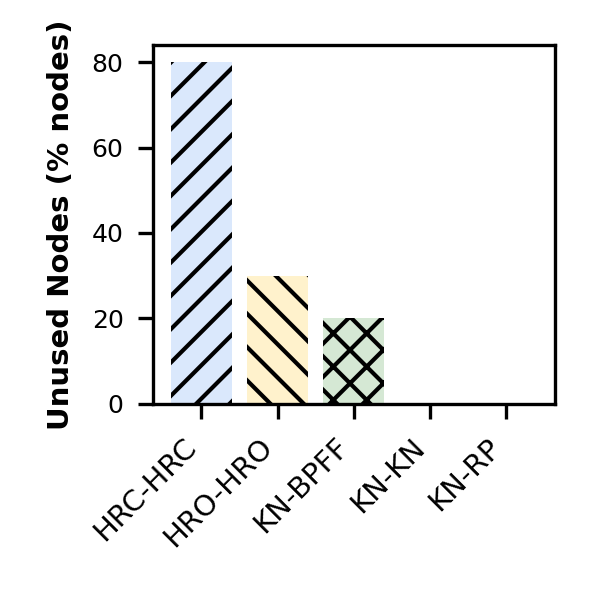
\includegraphics[width=0.155\linewidth]{6_Chapitre4/figures/eval/2-unused-nodes.png}
    }
    \subfloat[QoS\label{figure:herocache-evaluation-full-penalty}]{
        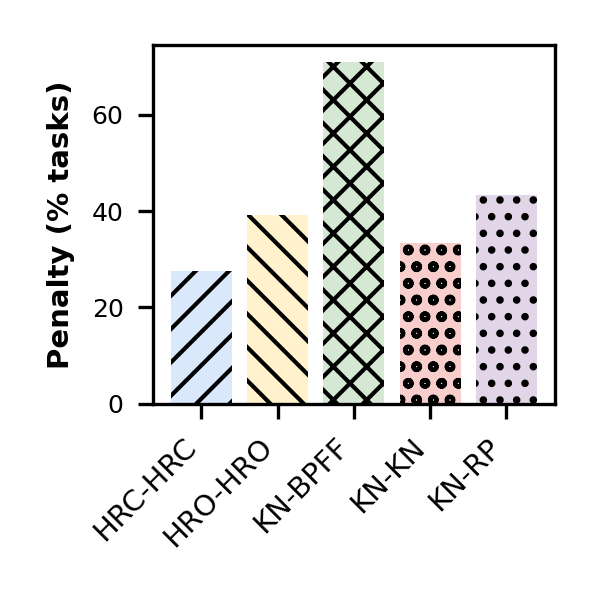
\includegraphics[width=0.155\linewidth]{6_Chapitre4/figures/eval/3-penalty-proportions.png}
    }
    \subfloat[Energy\label{figure:herocache-evaluation-full-energy-consumption}]{
        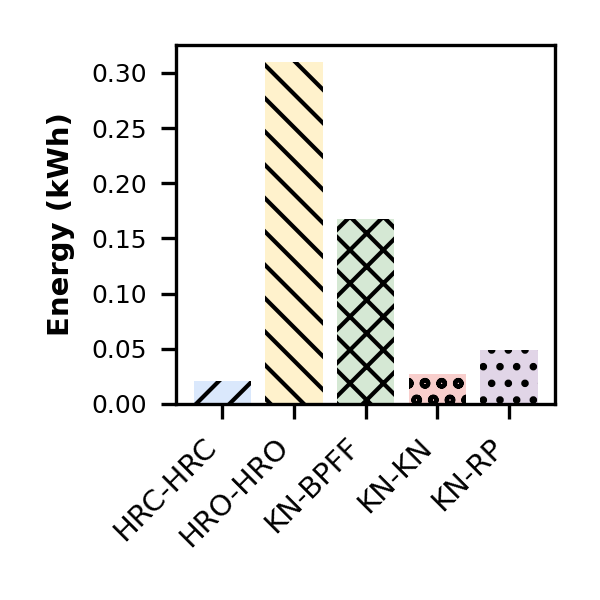
\includegraphics[width=0.155\linewidth]{6_Chapitre4/figures/eval/6-energy-consumption.png}
    }
    \subfloat[Consolidation\label{figure:herocache-evaluation-components-unused-nodes}]{
        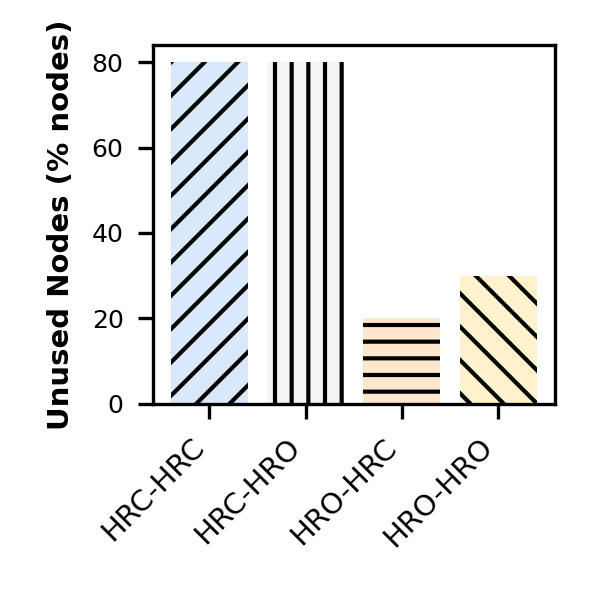
\includegraphics[width=0.155\linewidth]{6_Chapitre4/figures/eval-components/2-unused-nodes.png}
    }
    \subfloat[QoS\label{figure:herocache-evaluation-components-penalty}]{
        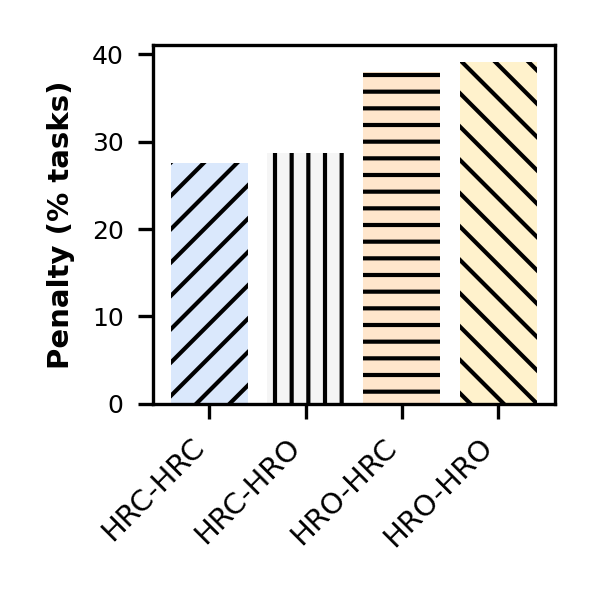
\includegraphics[width=0.155\linewidth]{6_Chapitre4/figures/eval-components/3-penalty-proportions.png}
    }
    \subfloat[Energy\label{figure:herocache-evaluation-components-energy-consumption}]{
        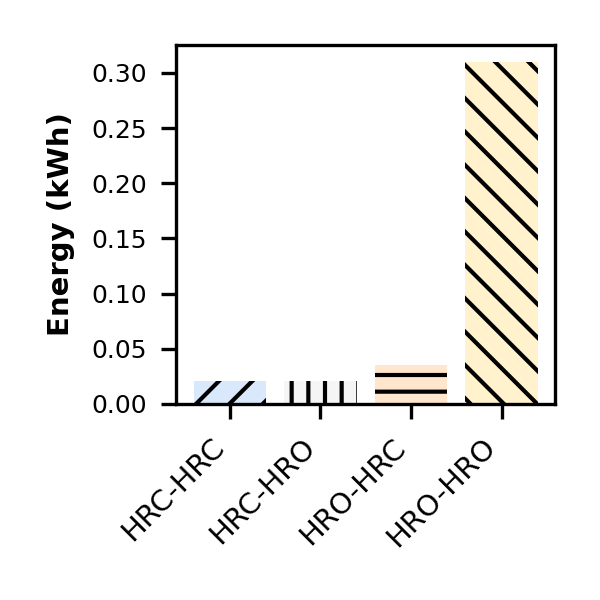
\includegraphics[width=0.155\linewidth]{6_Chapitre4/figures/eval-components/6-energy-consumption.png}
    }
    \caption{Evaluation -- Comparison against baselines (a-c) and impact of individual components (d-f)}
    \label{figure:herocache-evaluation}
\end{figure*}

\subsection{Protocole expérimental}

% \begin{figure}[t]
% \centering
% 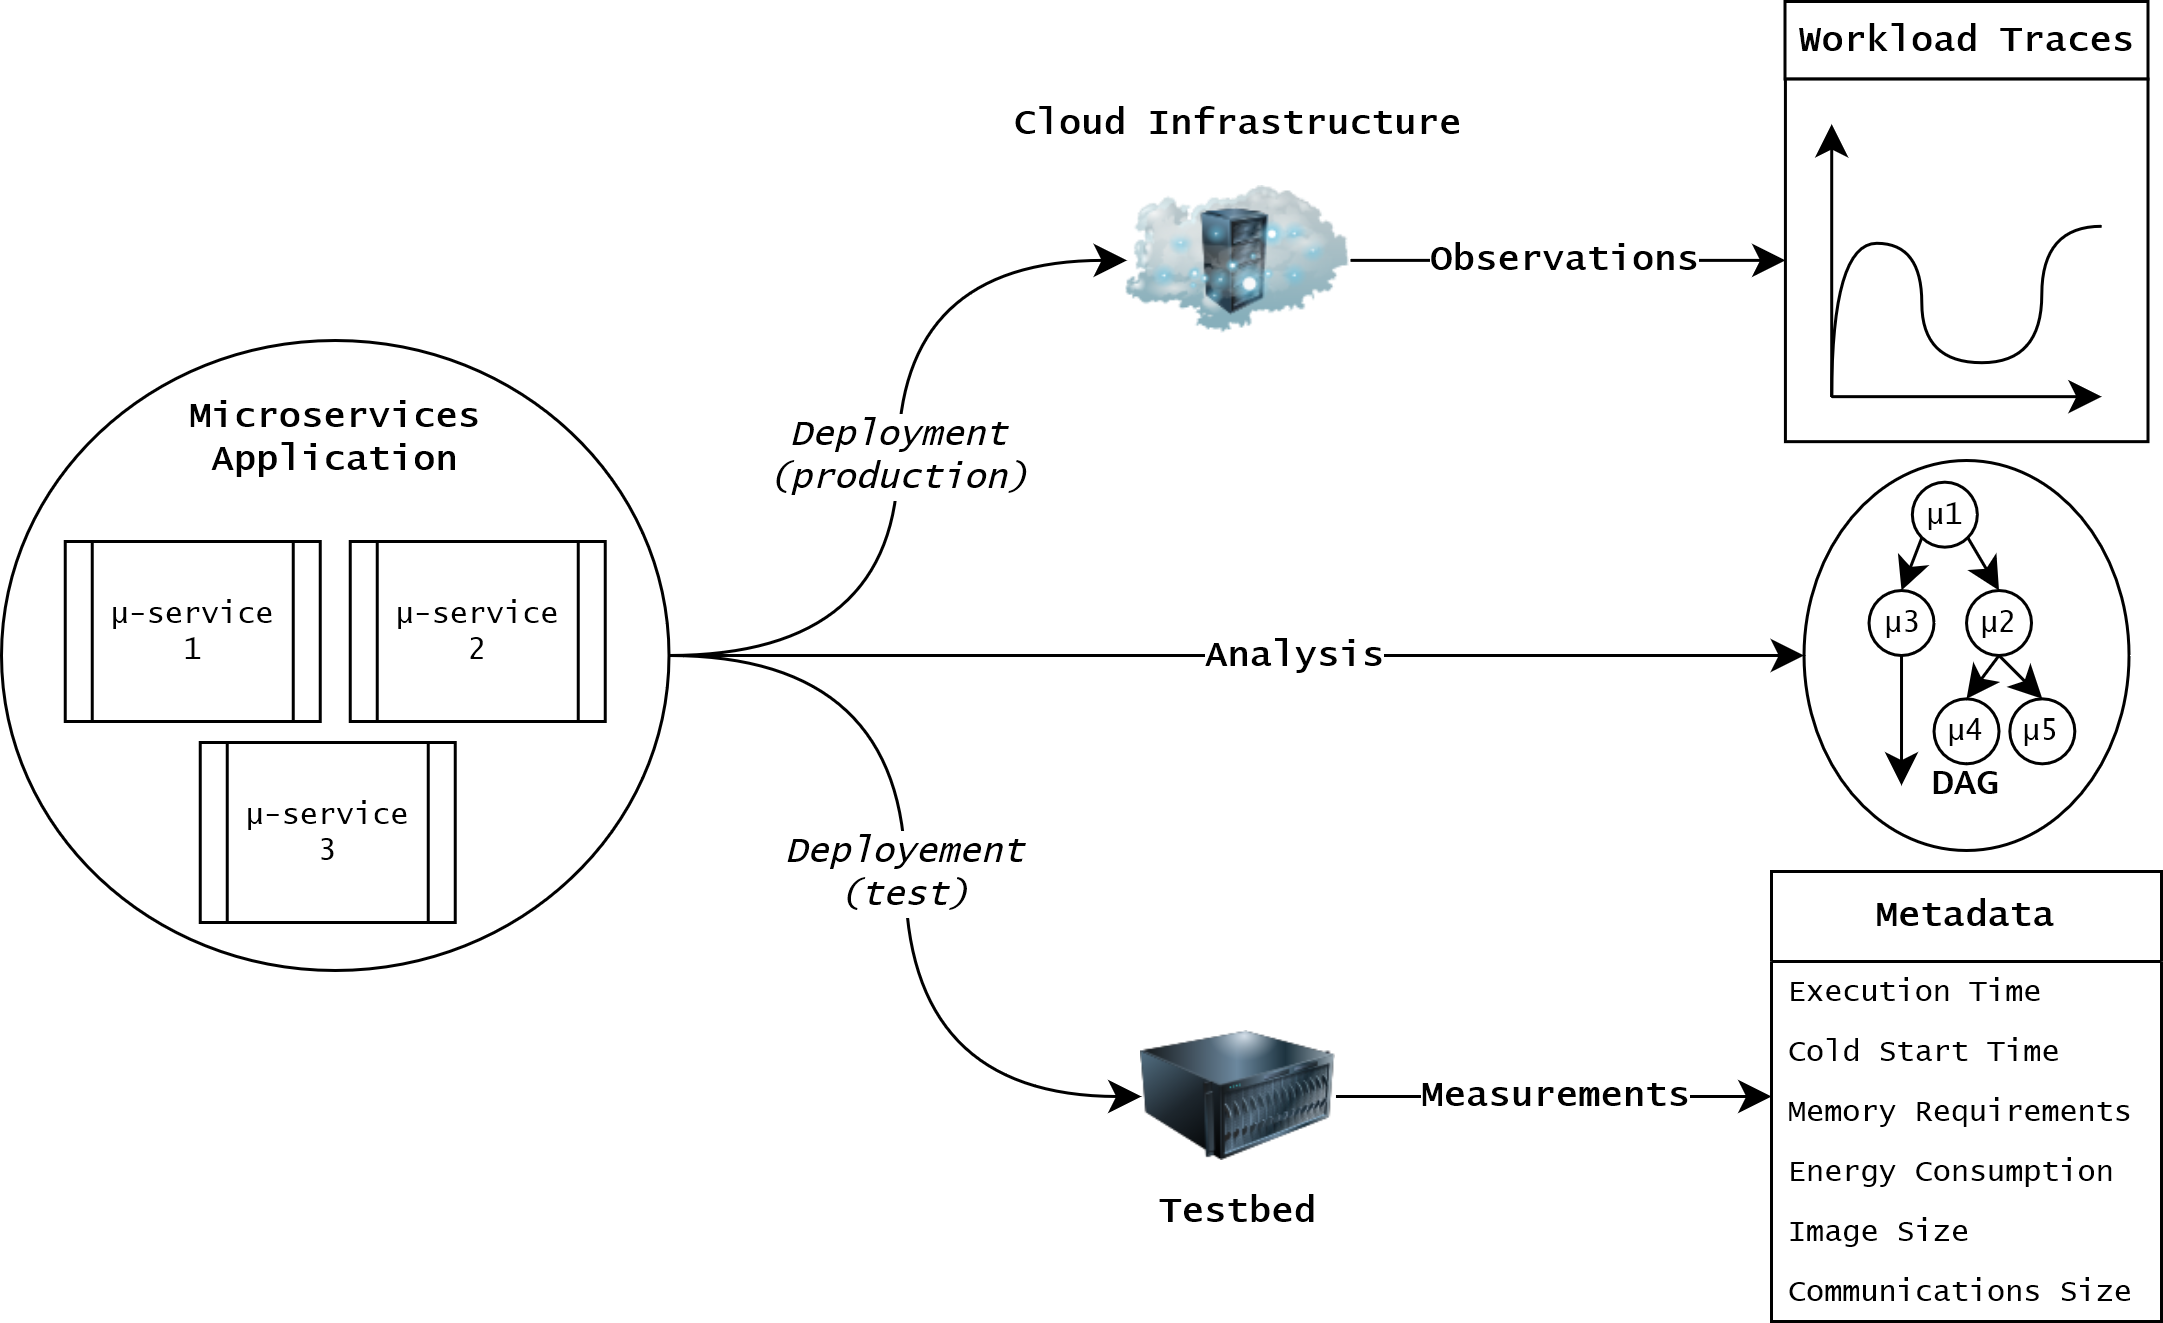
\includegraphics[width=\columnwidth]{6_Chapitre4/figures/use-case.png}
% \caption{Proposed methodology for workload characterization \vl{bon ben j'imagine qu'elle dégage aussi celle-là, vu la place qu'elle occupe...}}
% \label{figure:herocache-use-case}
% \end{figure}

\textbf{Offline characterization metadata}. To evaluate our contribution, we ran measurements for three IDS applications (see Section~\ref{section:herocache-characterization-workloads}). These applications consist of different preprocessing and inference functions that have been implemented on heterogeneous hardware (see Section~\ref{section:herocache-characterization-platforms}). These metadata served as input for a simulator~\footnote{\href{https://github.com/b-com/HeROsim}{https://github.com/b-com/HeROsim}} we built using SimPy~\cite{simpy}.

\textbf{Online scheduling}.
%Figure~\ref{figure:herocache-serverless-platform} summarizes our approach with respect to metadata collection. 
%As we were not able to deploy our IDS applications in a real-world setting to collect execution traces depicting end-users' usage,
We generated synthetic scenarios by modeling user requests as a Poisson process, following a uniform distribution across application invocations as devised in~\cite{9928755}. By tweaking the $\lambda$ parameter of the Poisson process, we can generate various traces with different rates of Requests per Second (RPS). We considered a scenario with 10 edge nodes communicating through 4G (LTE) connectivity. The bandwidth for 4G LTE depends on various factors ranging from antenna coverage, to communications service provider's QoS, to receiver quality. We chose to use broad values of 100 Mbps (12.5~MB/s). TCP packets to be analyzed are 1.5~KB size, and are sent in batches of 100 units to the IDS applications. This results in a rate of 83~RPS in our scenario, for 10 minutes of user requests. 

Weights for the autoscaling decisions (Equation~\ref{eq:herocache-scale-cost-function}) have been set to $k_{CP} = \frac{3}{8}$, $k_{TT} = \frac{3}{8}$, $k_{EC} = \frac{1}{8}$ and $k_{HP} = \frac{1}{8}$. Weights for the scheduling decisions (Equation~\ref{eq:herocache-scheduling-cost-function}) have been set to $k_{QP} = \frac{2}{3}$, $k_{EC} = \frac{0.5}{6}$ and $k_{TC} = \frac{1.5}{6}$. We use values inspired from \cite{herofake} so as to be comparable.

%To prevent a form of "thrashing" where replicas are created and destroyed in a loop when in-system concurrency is very close to the concurrency threshold, the autoscaler enforces a low keep-alive time that prevents the removal of a replica that was recently allocated. We set this keep-alive time at 30 seconds, which is the default value in Knative. \jb{could be removed if lack of space}

In our experiments, we make it possible to evaluate the autoscaler and the scheduler separately to better understand their behavior. We evaluated different combinations to show which part of each policy is relevant to address the various challenges in our problem. We implemented three autoscalers in our simulator:

\begin{itemize}
    \item HeROcache (HRC) -- Our autoscaling policy;% relies on function image caching on the edge nodes and tries to prefetch function images to satisfy dependencies ahead of deployment in the applications DAG;
    \item HeROfake (HRO)\cite{herofake} -- Enforces a policy similar to HRC, but is oblivious of storage costs; %: it does not use node-local image cache when instantiating function replicas, nor does it perform prefetching of function images based on their application's DAG;
    \item Knative (KN)~\cite{sureshENSUREEfficientScheduling2020}-- We modeled the Knative autoscaler behavior to the best of our knowledge. It deploys function replicas on the most available node.
\end{itemize}

On top of these autoscalers, we used four schedulers:

\begin{itemize}
    \item HeROcache (HRC) -- Our scheduling policy;% selects incoming user requests by earliest deadline first in order to maximize QoS. It factors in predicted communications latency and selects a replica based on response time requirements dictated by user request;
    \item HeROfake (HRO)~\cite{herofake} -- Enforces a policy similar to HRC, but is oblivious of storage costs;%: it does not predict communications latency in the application's DAG;
    \item Knative (KN)~\cite{knative} -- Knative considers execution platforms as homogeneous and does not enforce QoS. Replicas are sorted by in-flight requests count; the replica with the shortest queue is selected;
    \item Bin-Packing First Fit (BPFF)~\cite{wangPeekingCurtainsServerlessb} -- Tasks are consolidated on the minimum number of nodes and execution platforms. Nodes are sorted by available memory; the first function replica on a node with available memory will be selected for the user request. BPFF is likely to be the scheduling policy for AWS Lambda;
    \item Random Placement (RP) -- Tasks are scheduled on a randomly selected replica.
\end{itemize}

The naming of each scenario consists of two parts divided by a dash symbol. The first part corresponds to the autoscaling policy; the second part corresponds to the scheduling policy.% (for example, HRC-KN means we used the HeROcache autoscaler with the Knative scheduler).

We designed a two-step performance evaluation:\\
(1) \textbf{Comparison against baselines}: we compare full-featured HeROcache (HRC-HRC) to: (1) full-featured Knative (KN-KN), (2) full-featured HeROfake (HRO-HRO), (3) Knative autoscaler with BPFF scheduler (KN-BPFF), (4) Knative autoscaler with RP scheduler (KN-RP).\\
(2) \textbf{Impact of HeROcache components on the overall performance}: we discuss the individual impact of the autoscaler and the scheduler in different strategies: (1) HeROcache autoscaler with HeROfake scheduler (HRC-HRO), and (2) HeROfake autoscaler with HeROcache scheduler (HRO-HRC), comparing them to full-featured HeROcache and HeROfake.

We evaluate HeROcache on the basis of three  metrics: (1) the number of unused nodes in the infrastructure, which measures the consolidation level reached; (2) QoS penalties, which expresses the capability for our strategy to meet user requirements; (3) energy consumption, which is a salient challenge in resource-constrained edge computing.

\subsection{Analyse des résultats}

\subsubsection{Comparaison aux politiques de base}

\textbf{Tasks consolidation}. Figure~\ref{figure:herocache-evaluation-full-unused-nodes} shows that our combination of autoscaler and scheduler achieves the best task consolidation, utilizing only 20\% of the edge infrastructure for the execution of the scenario. Knative behaves as expected, spreading the load across the entire infrastructure. Note that BPFF under Knative produces slightly different results: as task queues are maximized, the autoscaler does not need to allocate as many replicas. In this scenario, if the unused edge nodes were powered off instead of sitting idle, our strategy would allow the service provider to save almost 100 Wh (that is 80\% of the static energy and more than 83\% of the total energy) by turning off 80\% of the infrastructure, while still guaranteeing the application response time for 72\% of user requests.

\textbf{Quality of Service}. Figure~\ref{figure:herocache-evaluation-full-penalty} illustrates how relevant taking resources heterogeneity into account is. Indeed, our policy manages to keep QoS violations at 27.5\% while leaving 80\% of the infrastructure unused. Knative violates just over 30\% of the user requests QoS while spreading the load over all the available edge nodes, which is counterintuitive. This is explained by the dependencies between tasks that Knative does not take into account. As a consequence, tasks communicate over slow network storage. While tasks in Knative may spend less time in queue, they still exhibit higher latency than in HeROcache. When using the BPFF policy, violations go up to almost 70\%: in this situation, replica queues are too long for tasks to complete within their deadline. For comparison's sake, Knative using the RP scheduler keeps QoS violations around 50\%. HeROfake generates 39\% QoS violations.

Our policy keeps the proportion of cold starts below 0.011\% of user requests, whereas Knative suffers from 4 times more cold starts. In HeROcache, node-local image cache is hit in 33\% of function initializations, reducing initialization delays by 17.6\%.
With HeROcache, 30\% of the tasks manage to communicate through node-local storage, speeding up application execution by reducing communications latency by 88.4\%.

\textbf{Energy consumption}. Figure~\ref{figure:herocache-evaluation-full-energy-consumption} shows that HeROcache manages to cut dynamic energy consumption by a third: with a makespan of 1505 seconds for the scenario, the infrastructure consumes 0.0088 kWh, as compared to 0.0266 kWh for 2193 seconds of execution time under Knative. Not only does HeROcache's consolidation strategy allow for power-off policies that could provide important reductions in static energy requirements for running IDS applications on the edge, but by selecting adequate execution platforms, it also reduces the overall consumption of the edge cluster. HeROfake consumes the most energy at 0.31 kWh because of a much longer execution time for the scenario.

\subsubsection{Impact des composants individuels}

\textbf{Tasks consolidation}. Figure~\ref{figure:herocache-evaluation-components-unused-nodes} shows that strategies that are oblivious to storage costs do not manage to consolidate tasks as well as HeROcache: HRO-HRC and HRO-HRO respectively use 80\% and 70\% of the infrastructure. We explain these results as follows: as dependencies are not satisfied in time, load keeps on growing for the various functions, leading the autoscaler to increase the number of replicas, thus enroling more nodes for the duration of the scenario.%: HRO-HRC uses 80\% of the infrastructure.

\textbf{Quality of Service}. Figure~\ref{figure:herocache-evaluation-components-penalty} illustrates the consequence of the previous point: QoS penalties are higher with an autoscaler that does not factor in the delays introduced by function image pulling and function communications. While HRO-HRC is indeed aware of hardware and request heterogeneity, it still finishes at 37.9\% of applications missing their deadline.

\textbf{Energy consumption}. Figure~\ref{figure:herocache-evaluation-components-energy-consumption} displays that while HRO-HRC allocates 70\% of the infrastructure, it still manages to keep energy consumption almost as low as HRC-HRC. This is because it chose the nodes that were the least energy-hungry, at the expense of penalties that it could not predict since it is not storage-aware.

\textbf{Note on complexity}: HeROcache employs a greedy optimization technique comparable to HeROfake. In HeROcache, the complexity is bounded by the number of applications $A$, their size $f_{a}$ and the size of the infrastructure $N$ (Equation~\ref{eq:herocache-complexity-autoscaler}): in the worst-case scenario where all the resources are available, the autoscaler scans through the whole infrastructure $N$ to score each node for replica creation.

\begin{equation}
    \mathcal{O}_{autoscaling}(A \cdot f_{a} \cdot N)
\label{eq:herocache-complexity-autoscaler}
\end{equation}

As the scheduler works with already created replicas $R_{f}$ of functions, its complexity is lower (Equation~\ref{eq:herocache-complexity-scheduler}).

\begin{equation}
    \mathcal{O}_{scheduling}(A \cdot f_{a} \cdot R_{f})
\label{eq:herocache-complexity-scheduler}
\end{equation}

As our current case study implies a limited subset of IDS functions with a reasonable number of edge nodes, the scalability was not an issue. However, this overhead should be considered for wider deployments of different case studies.
%These overheads have not been measured in simulation. However, as the autoscaler works in a periodic fashion, the frequency of the period could be tuned to adjust the algorithm depending on the service provider's needs. The scheduler is called at the time of user requests and could be distributed across nodes if the load is too heavy to handle.

\section{Travaux connexes}
\label{section:herocache-sota}

Previous work focused on autoscaling platforms for the deployment of short-lived tasks, comprised in applications exhibiting unpredictable load patterns (see Table~\ref{table:herocache-sota}).% summarizes how these contributions differ from our target solution.

%Among these works, 
\cite{smithFaDOFaaSFunctions2022} proposes a data-aware orchestrator, but does not consider the snowballing of delays across function chains. \cite{zhangFIRSTExploitingMultiDimensional2023} does not support the scheduling of these function chains.
All of these contributions consider a homogeneous infrastructure \cite{bhasiCypressInputSizesensitive2022, zijunFassflowEfficient2022, smithFaDOFaaSFunctions2022, zhangFIRSTExploitingMultiDimensional2023, abdiPaletteLoadBalancing2023}. This is not representative of our use case, where edge devices are highly heterogeneous. HeROfake~\cite{herofake} %\footnote{As this is the only work targeting heterogeneous devices (but for another type of applications), we named our own strategy with a similar name to emphasize this aspect of our contribution}
leverages hardware heterogeneity in their orchestration policy, but does not integrate inter-function dependencies nor image caching in their cost model. It was chosen for evaluation purposes to highlight the need to consider such costs. %and therefore does not perform as well as HeROcache for the orchestration of function chains.
Some of these contributions optimize energy consumption at the autoscaler level \cite{bhasiCypressInputSizesensitive2022, zhangFIRSTExploitingMultiDimensional2023}. However, they focus on the dynamic part of energy consumption: they do not consider the possible impact of consolidation towards static energy consumption. We argue that service providers should seek task consolidation as a means to power off as many nodes as possible, dramatically lowering the overall infrastructure energy requirements.
In \cite{fuerstIluvatarFastControl2023}, the authors investigated the various overheads inflicted by serverless orchestration. This element has not been taken into account in our study, as we are targeting an edge infrastructure limited in size for the deployment of a single application.

\section{Conclusion et perspectives}
\label{section:herocache-conclusion}

In this work, we presented an allocation and scheduling policy for serverless edge computing. This policy seeks to optimize time-sensitive applications deployment for QoS on energy-constrained devices. By leveraging workload characterization, hardware heterogeneity and local storage devices on the edge nodes, HeROcache enforces applications consolidation and manages to reduce average initialization delays by 17.6\% and communication delays by 88.4\%. This results in reducing the static energy consumption of the platform by 80\% while maintaining under 28\% of QoS violations. We plan to generalize the HeROcache approach for case studies including several types of application on larger edge or cloud infrastructures. For such a sake, machine learning strategies or metaheuristics could be used for scaling purposes.
